% **************************************************************************************************************
% A Classic Thesis Style
% An Homage to The Elements of Typographic Style
%
% Copyright (C) 2015 André Miede http://www.miede.de
%
% If you like the style then I would appreciate a postcard. My address 
% can be found in the file ClassicThesis.pdf. A collection of the 
% postcards I received so far is available online at 
% http://postcards.miede.de
%
% License:
% This program is free software; you can redistribute it and/or modify
% it under the terms of the GNU General Public License as published by
% the Free Software Foundation; either version 2 of the License, or
% (at your option) any later version.
%
% This program is distributed in the hope that it will be useful,
% but WITHOUT ANY WARRANTY; without even the implied warranty of
% MERCHANTABILITY or FITNESS FOR A PARTICULAR PURPOSE.  See the
% GNU General Public License for more details.
%
% You should have received a copy of the GNU General Public License
% along with this program; see the file COPYING.  If not, write to
% the Free Software Foundation, Inc., 59 Temple Place - Suite 330,
% Boston, MA 02111-1307, USA.
%
% **************************************************************************************************************
\RequirePackage{fix-cm} % fix some latex issues see: http://texdoc.net/texmf-dist/doc/latex/base/fixltx2e.pdf
\documentclass[ twoside,openright,titlepage,numbers=noenddot,headinclude,%1headlines,% letterpaper a4paper
                footinclude=true,cleardoublepage=empty,abstractoff, % <--- obsolete, remove (todo)
                BCOR=5mm,paper=a4,fontsize=11pt,%11pt,a4paper,%
                ngerman,american,%
                ]{scrreprt}

%********************************************************************
% Note: Make all your adjustments in here
%*******************************************************
% ****************************************************************************************************
% classicthesis-config.tex 
% formerly known as loadpackages.sty, classicthesis-ldpkg.sty, and classicthesis-preamble.sty 
% Use it at the beginning of your ClassicThesis.tex, or as a LaTeX Preamble 
% in your ClassicThesis.{tex,lyx} with % ****************************************************************************************************
% classicthesis-config.tex 
% formerly known as loadpackages.sty, classicthesis-ldpkg.sty, and classicthesis-preamble.sty 
% Use it at the beginning of your ClassicThesis.tex, or as a LaTeX Preamble 
% in your ClassicThesis.{tex,lyx} with % ****************************************************************************************************
% classicthesis-config.tex 
% formerly known as loadpackages.sty, classicthesis-ldpkg.sty, and classicthesis-preamble.sty 
% Use it at the beginning of your ClassicThesis.tex, or as a LaTeX Preamble 
% in your ClassicThesis.{tex,lyx} with \input{classicthesis-config}
% ****************************************************************************************************  
% If you like the classicthesis, then I would appreciate a postcard. 
% My address can be found in the file ClassicThesis.pdf. A collection 
% of the postcards I received so far is available online at 
% http://postcards.miede.de
% ****************************************************************************************************


% ****************************************************************************************************
% 0. Set the encoding of your files. UTF-8 is the only sensible encoding nowadays. If you can't read
% äöüßáéçèê∂åëæƒÏ€ then change the encoding setting in your editor, not the line below. If your editor
% does not support utf8 use another editor!
% ****************************************************************************************************
\PassOptionsToPackage{utf8}{inputenc}
\usepackage{inputenc}
        
% ****************************************************************************************************
% 1. Configure classicthesis for your needs here, e.g., remove "drafting" below 
% in order to deactivate the time-stamp on the pages
% ****************************************************************************************************
\PassOptionsToPackage{eulerchapternumbers,listings,%drafting,%
					 pdfspacing,%floatperchapter,%linedheaders,%
					 subfig,beramono,eulermath,parts}{classicthesis}                                        
% ********************************************************************
% Available options for classicthesis.sty 
% (see ClassicThesis.pdf for more information):
% drafting
% parts nochapters linedheaders
% eulerchapternumbers beramono eulermath pdfspacing minionprospacing
% tocaligned dottedtoc manychapters
% listings floatperchapter subfig
% ********************************************************************

\usepackage{url}
\usepackage{nameref}
\usepackage{datetime} %needed to add the date just below
% ****************************************************************************************************
% 2. Personal data and user ad-hoc commands
% ****************************************************************************************************
\newcommand{\myTitle}{Remote Monitoring of Health Parameters\xspace}
\newcommand{\mySubtitle}{Using Smart Walker\xspace}
\newcommand{\myDegree}{Project Report\xspace}
\newcommand{\myNameP}{Patrick Lewandowski\xspace}
\newcommand{\myStudentIdP}{201802946\xspace}
\newcommand{\myNameH}{Harshit Mahapatra\xspace}
\newcommand{\myStudentIdH}{201803187\xspace}
\newcommand{\myNameT}{Tomas Manuel Rebelo Mota\xspace}
\newcommand{\myStudentIdT}{201802941\xspace}
\newcommand{\myProf}{Niels Olof Bouvin\xspace}
\newcommand{\myOtherProf}{Michal Ratajský\xspace}
\newcommand{\mySupervisor}{Put name here\xspace}
\newcommand{\myFaculty}{Science \& Technology\xspace}
\newcommand{\myDepartment}{Department of Computer Science\xspace}
\newcommand{\myUni}{Aarhus University\xspace}
\newcommand{\myLocation}{Aarhus\xspace}
\newcommand{\myTime}{\monthname\ \the\year\xspace}
\newcommand{\myVersion}{\xspace}


% ********************************************************************
% Setup, finetuning, and useful commands
% ********************************************************************
\newcounter{dummy} % necessary for correct hyperlinks (to index, bib, etc.)
\newlength{\abcd} % for ab..z string length calculation
\providecommand{\mLyX}{L\kern-.1667em\lower.25em\hbox{Y}\kern-.125emX\@}
\providecommand{\mBibTeX}{\textsc{Bib}\negthinspace\TeX\@}
% ****************************************************************************************************


% ****************************************************************************************************
% 3. Loading some handy packages
% ****************************************************************************************************
% ******************************************************************** 
% Packages with options that might require adjustments
% ******************************************************************** 
%\PassOptionsToPackage{ngerman,american}{babel}   % change this to your language(s)
% Spanish languages need extra options in order to work with this template
%\PassOptionsToPackage{spanish,es-lcroman}{babel}
\usepackage[american]{babel}                  
\usepackage{microtype}
\usepackage{csquotes}
\usepackage{ragged2e}
\usepackage[dvipsnames]{xcolor}
\usepackage{pgf-umlsd}
\usepackage{pgfplots}
\usepackage{pgfplotstable}
% recommended:
\usepackage{booktabs}
\usepackage{array}
\usepackage{colortbl}
% \usepackage{color}
\definecolor{aublue}{HTML}{193b77} % the dark blue colour used by AU



%\usepackage[square,numbers,sort&compress]{natbib}
%\bibliographystyle{abbrvnat}

\PassOptionsToPackage{%
   backend=biber, %instead of bibtex
	%backend=bibtex8,
	bibencoding=ascii,%
	language=auto,%
	style=numeric-comp,%
   %style=authoryear-comp, % Author 1999, 2010
   %bibstyle=authoryear,dashed=false, % dashed: substitute rep. author with ---
   sorting=nyt, % name, year, title
   maxbibnames=10, % default: 3, et al.
   %backref=true,%
   natbib=true % natbib compatibility mode (\citep and \citet still work)
}{biblatex}
\usepackage{biblatex}

\PassOptionsToPackage{fleqn}{amsmath}       % math environments and more by the AMS 
\usepackage{amsmath}
%
% ******************************************************************** 
% General useful packages
% ******************************************************************** 
\PassOptionsToPackage{T1}{fontenc} % T2A for cyrillics
\usepackage{fontenc}     
\usepackage{textcomp} % fix warning with missing font shapes
\usepackage{scrhack} % fix warnings when using KOMA with listings package          
\usepackage{xspace} % to get the spacing after macros right  
\newcommand{\eg}{e.g.,\xspace}
\newcommand{\Eg}{E.g.,\xspace}
\newcommand{\etal}{et~al.\xspace}
\newcommand{\etc}{etc.\@\xspace}
\newcommand{\ie}{i.e.,\xspace}
\newcommand{\viz}{viz.\@\xspace}

\usepackage{mparhack} % get marginpar right
\usepackage{fixltx2e} % fixes some LaTeX stuff --> since 2015 in the LaTeX kernel (see below)
%\usepackage[latest]{latexrelease} % will be used once available in more distributions (ISSUE #107)
\PassOptionsToPackage{printonlyused,smaller}{acronym} 
    \usepackage{acronym} % nice macros for handling all acronyms in the thesis
    %\renewcommand{\bflabel}[1]{{#1}\hfill} % fix the list of acronyms --> no longer working
    %\renewcommand*{\acsfont}[1]{\textsc{#1}} 
    \renewcommand*{\aclabelfont}[1]{\acsfont{#1}}
% ****************************************************************************************************


% ****************************************************************************************************
% 4. Setup floats: tables, (sub)figures, and captions
% ****************************************************************************************************
\usepackage{tabularx} % better tables
    \setlength{\extrarowheight}{3pt} % increase table row height
\newcommand{\tableheadline}[1]{\multicolumn{1}{c}{\spacedlowsmallcaps{#1}}}
\newcommand{\myfloatalign}{\centering} % to be used with each float for alignment
\usepackage{caption}
% Thanks to cgnieder and Claus Lahiri
% http://tex.stackexchange.com/questions/69349/spacedlowsmallcaps-in-caption-label
% [REMOVED DUE TO OTHER PROBLEMS, SEE ISSUE #82]    
%\DeclareCaptionLabelFormat{smallcaps}{\bothIfFirst{#1}{~}\MakeTextLowercase{\textsc{#2}}}
%\captionsetup{font=small,labelformat=smallcaps} % format=hang,
\captionsetup{font=small} % format=hang,
\usepackage{subfig}  
% ****************************************************************************************************


% ****************************************************************************************************
% 5. Setup code listings
% ****************************************************************************************************
\usepackage{listings} 
%\lstset{emph={trueIndex,root},emphstyle=\color{BlueViolet}}%\underbar} % for special keywords
\lstset{language=[LaTeX]Tex,%C++,
    morekeywords={PassOptionsToPackage,selectlanguage},
    keywordstyle=\color{RoyalBlue},%\bfseries,
    basicstyle=\small\ttfamily,
    identifierstyle=\color{NavyBlue},
    commentstyle=\color{Green}\ttfamily,
    stringstyle=\rmfamily,
    numbers=left,
    numberstyle=\tiny\color{Gray},
    stepnumber=1,
    numbersep=8pt,
    showstringspaces=false,
    breaklines=true,
    %frameround=ftff,
    %frame=single,
    belowcaptionskip=.75\baselineskip
    %frame=L
} 
% ****************************************************************************************************             


% ****************************************************************************************************
% 6. PDFLaTeX, hyperreferences and citation backreferences
% ****************************************************************************************************
% ********************************************************************
% Using PDFLaTeX
% ********************************************************************
\PassOptionsToPackage{pdftex,hyperfootnotes=false,pdfpagelabels}{hyperref}
    \usepackage{hyperref}  % backref linktocpage pagebackref
\pdfcompresslevel=9
\pdfadjustspacing=1 
\PassOptionsToPackage{pdftex}{graphicx}
    \usepackage{graphicx} 
 

% ********************************************************************
% Hyperreferences
% ********************************************************************
\hypersetup{%
    %draft, % = no hyperlinking at all (useful in b/w printouts)
    colorlinks=true, linktocpage=true, pdfstartpage=3, pdfstartview=FitV,%
    % uncomment the following line if you want to have black links (e.g., for printing)
    %colorlinks=false, linktocpage=false, pdfstartpage=3, pdfstartview=FitV, pdfborder={0 0 0},%
    breaklinks=true, pdfpagemode=UseNone, pageanchor=true, pdfpagemode=UseOutlines,%
    plainpages=false, bookmarksnumbered, bookmarksopen=true, bookmarksopenlevel=1,%
    hypertexnames=true, pdfhighlight=/O,%nesting=true,%frenchlinks,%
    urlcolor=webbrown, linkcolor=RoyalBlue, citecolor=webgreen, %pagecolor=RoyalBlue,%
    %urlcolor=Black, linkcolor=Black, citecolor=Black, %pagecolor=Black,%
    pdftitle={\myTitle},%
    pdfauthor={\textcopyright\ \myNameP, \myNameH, \myNameT \myUni, \myFaculty},%
    pdfsubject={},%
    pdfkeywords={},%
    pdfcreator={pdfLaTeX},%
    pdfproducer={LaTeX with hyperref and classicthesis}%
}   

% ********************************************************************
% Setup autoreferences
% ********************************************************************
% There are some issues regarding autorefnames
% http://www.ureader.de/msg/136221647.aspx
% http://www.tex.ac.uk/cgi-bin/texfaq2html?label=latexwords
% you have to redefine the makros for the 
% language you use, e.g., american, ngerman
% (as chosen when loading babel/AtBeginDocument)
% ********************************************************************
\makeatletter
\@ifpackageloaded{babel}%
    {%
       \addto\extrasamerican{%
			\renewcommand*{\figureautorefname}{Figure}%
			\renewcommand*{\tableautorefname}{Table}%
			\renewcommand*{\partautorefname}{Part}%
			\renewcommand*{\chapterautorefname}{Chapter}%
			\renewcommand*{\sectionautorefname}{Section}%
			\renewcommand*{\subsectionautorefname}{Section}%
			\renewcommand*{\subsubsectionautorefname}{Section}%     
                }%
       \addto\extrasngerman{% 
			\renewcommand*{\paragraphautorefname}{Absatz}%
			\renewcommand*{\subparagraphautorefname}{Unterabsatz}%
			\renewcommand*{\footnoteautorefname}{Fu\"snote}%
			\renewcommand*{\FancyVerbLineautorefname}{Zeile}%
			\renewcommand*{\theoremautorefname}{Theorem}%
			\renewcommand*{\appendixautorefname}{Anhang}%
			\renewcommand*{\equationautorefname}{Gleichung}%        
			\renewcommand*{\itemautorefname}{Punkt}%
                }%  
            % Fix to getting autorefs for subfigures right (thanks to Belinda Vogt for changing the definition)
            \providecommand{\subfigureautorefname}{\figureautorefname}%             
    }{\relax}
\makeatother


% ****************************************************************************************************
% 7. Last calls before the bar closes
% ****************************************************************************************************
% ********************************************************************
% Development Stuff
% ********************************************************************
\listfiles
%\PassOptionsToPackage{l2tabu,orthodox,abort}{nag}
%   \usepackage{nag}
%\PassOptionsToPackage{warning, all}{onlyamsmath}
%   \usepackage{onlyamsmath}

% ********************************************************************
% Last, but not least...
% ********************************************************************
\usepackage{classicthesis} 
% ****************************************************************************************************


% ****************************************************************************************************
% 8. Further adjustments (experimental)
% ****************************************************************************************************
% ********************************************************************
% Changing the text area
% ********************************************************************
%\linespread{1.05} % a bit more for Palatino
%\areaset[current]{312pt}{761pt} % 686 (factor 2.2) + 33 head + 42 head \the\footskip
%\setlength{\marginparwidth}{7em}%
%\setlength{\marginparsep}{2em}%

% ********************************************************************
% Using different fonts
% ********************************************************************
%\usepackage[oldstylenums]{kpfonts} % oldstyle notextcomp
%\usepackage[osf]{libertine}
%\usepackage[light,condensed,math]{iwona}
%\renewcommand{\sfdefault}{iwona}
%\usepackage{lmodern} % <-- no osf support :-(
%\usepackage{cfr-lm} % 
%\usepackage[urw-garamond]{mathdesign} <-- no osf support :-(
%\usepackage[default,osfigures]{opensans} % scale=0.95 
%\usepackage[sfdefault]{FiraSans}
% ****************************************************************************************************



%%% Local Variables:
%%% mode: latex
%%% TeX-master: "./ClassicThesis"
%%% End:

% ****************************************************************************************************  
% If you like the classicthesis, then I would appreciate a postcard. 
% My address can be found in the file ClassicThesis.pdf. A collection 
% of the postcards I received so far is available online at 
% http://postcards.miede.de
% ****************************************************************************************************


% ****************************************************************************************************
% 0. Set the encoding of your files. UTF-8 is the only sensible encoding nowadays. If you can't read
% äöüßáéçèê∂åëæƒÏ€ then change the encoding setting in your editor, not the line below. If your editor
% does not support utf8 use another editor!
% ****************************************************************************************************
\PassOptionsToPackage{utf8}{inputenc}
\usepackage{inputenc}
        
% ****************************************************************************************************
% 1. Configure classicthesis for your needs here, e.g., remove "drafting" below 
% in order to deactivate the time-stamp on the pages
% ****************************************************************************************************
\PassOptionsToPackage{eulerchapternumbers,listings,%drafting,%
					 pdfspacing,%floatperchapter,%linedheaders,%
					 subfig,beramono,eulermath,parts}{classicthesis}                                        
% ********************************************************************
% Available options for classicthesis.sty 
% (see ClassicThesis.pdf for more information):
% drafting
% parts nochapters linedheaders
% eulerchapternumbers beramono eulermath pdfspacing minionprospacing
% tocaligned dottedtoc manychapters
% listings floatperchapter subfig
% ********************************************************************

\usepackage{url}
\usepackage{nameref}
\usepackage{datetime} %needed to add the date just below
% ****************************************************************************************************
% 2. Personal data and user ad-hoc commands
% ****************************************************************************************************
\newcommand{\myTitle}{Remote Monitoring of Health Parameters\xspace}
\newcommand{\mySubtitle}{Using Smart Walker\xspace}
\newcommand{\myDegree}{Project Report\xspace}
\newcommand{\myNameP}{Patrick Lewandowski\xspace}
\newcommand{\myStudentIdP}{201802946\xspace}
\newcommand{\myNameH}{Harshit Mahapatra\xspace}
\newcommand{\myStudentIdH}{201803187\xspace}
\newcommand{\myNameT}{Tomas Manuel Rebelo Mota\xspace}
\newcommand{\myStudentIdT}{201802941\xspace}
\newcommand{\myProf}{Niels Olof Bouvin\xspace}
\newcommand{\myOtherProf}{Michal Ratajský\xspace}
\newcommand{\mySupervisor}{Put name here\xspace}
\newcommand{\myFaculty}{Science \& Technology\xspace}
\newcommand{\myDepartment}{Department of Computer Science\xspace}
\newcommand{\myUni}{Aarhus University\xspace}
\newcommand{\myLocation}{Aarhus\xspace}
\newcommand{\myTime}{\monthname\ \the\year\xspace}
\newcommand{\myVersion}{\xspace}


% ********************************************************************
% Setup, finetuning, and useful commands
% ********************************************************************
\newcounter{dummy} % necessary for correct hyperlinks (to index, bib, etc.)
\newlength{\abcd} % for ab..z string length calculation
\providecommand{\mLyX}{L\kern-.1667em\lower.25em\hbox{Y}\kern-.125emX\@}
\providecommand{\mBibTeX}{\textsc{Bib}\negthinspace\TeX\@}
% ****************************************************************************************************


% ****************************************************************************************************
% 3. Loading some handy packages
% ****************************************************************************************************
% ******************************************************************** 
% Packages with options that might require adjustments
% ******************************************************************** 
%\PassOptionsToPackage{ngerman,american}{babel}   % change this to your language(s)
% Spanish languages need extra options in order to work with this template
%\PassOptionsToPackage{spanish,es-lcroman}{babel}
\usepackage[american]{babel}                  
\usepackage{microtype}
\usepackage{csquotes}
\usepackage{ragged2e}
\usepackage[dvipsnames]{xcolor}
\usepackage{pgf-umlsd}
\usepackage{pgfplots}
\usepackage{pgfplotstable}
% recommended:
\usepackage{booktabs}
\usepackage{array}
\usepackage{colortbl}
% \usepackage{color}
\definecolor{aublue}{HTML}{193b77} % the dark blue colour used by AU



%\usepackage[square,numbers,sort&compress]{natbib}
%\bibliographystyle{abbrvnat}

\PassOptionsToPackage{%
   backend=biber, %instead of bibtex
	%backend=bibtex8,
	bibencoding=ascii,%
	language=auto,%
	style=numeric-comp,%
   %style=authoryear-comp, % Author 1999, 2010
   %bibstyle=authoryear,dashed=false, % dashed: substitute rep. author with ---
   sorting=nyt, % name, year, title
   maxbibnames=10, % default: 3, et al.
   %backref=true,%
   natbib=true % natbib compatibility mode (\citep and \citet still work)
}{biblatex}
\usepackage{biblatex}

\PassOptionsToPackage{fleqn}{amsmath}       % math environments and more by the AMS 
\usepackage{amsmath}
%
% ******************************************************************** 
% General useful packages
% ******************************************************************** 
\PassOptionsToPackage{T1}{fontenc} % T2A for cyrillics
\usepackage{fontenc}     
\usepackage{textcomp} % fix warning with missing font shapes
\usepackage{scrhack} % fix warnings when using KOMA with listings package          
\usepackage{xspace} % to get the spacing after macros right  
\newcommand{\eg}{e.g.,\xspace}
\newcommand{\Eg}{E.g.,\xspace}
\newcommand{\etal}{et~al.\xspace}
\newcommand{\etc}{etc.\@\xspace}
\newcommand{\ie}{i.e.,\xspace}
\newcommand{\viz}{viz.\@\xspace}

\usepackage{mparhack} % get marginpar right
\usepackage{fixltx2e} % fixes some LaTeX stuff --> since 2015 in the LaTeX kernel (see below)
%\usepackage[latest]{latexrelease} % will be used once available in more distributions (ISSUE #107)
\PassOptionsToPackage{printonlyused,smaller}{acronym} 
    \usepackage{acronym} % nice macros for handling all acronyms in the thesis
    %\renewcommand{\bflabel}[1]{{#1}\hfill} % fix the list of acronyms --> no longer working
    %\renewcommand*{\acsfont}[1]{\textsc{#1}} 
    \renewcommand*{\aclabelfont}[1]{\acsfont{#1}}
% ****************************************************************************************************


% ****************************************************************************************************
% 4. Setup floats: tables, (sub)figures, and captions
% ****************************************************************************************************
\usepackage{tabularx} % better tables
    \setlength{\extrarowheight}{3pt} % increase table row height
\newcommand{\tableheadline}[1]{\multicolumn{1}{c}{\spacedlowsmallcaps{#1}}}
\newcommand{\myfloatalign}{\centering} % to be used with each float for alignment
\usepackage{caption}
% Thanks to cgnieder and Claus Lahiri
% http://tex.stackexchange.com/questions/69349/spacedlowsmallcaps-in-caption-label
% [REMOVED DUE TO OTHER PROBLEMS, SEE ISSUE #82]    
%\DeclareCaptionLabelFormat{smallcaps}{\bothIfFirst{#1}{~}\MakeTextLowercase{\textsc{#2}}}
%\captionsetup{font=small,labelformat=smallcaps} % format=hang,
\captionsetup{font=small} % format=hang,
\usepackage{subfig}  
% ****************************************************************************************************


% ****************************************************************************************************
% 5. Setup code listings
% ****************************************************************************************************
\usepackage{listings} 
%\lstset{emph={trueIndex,root},emphstyle=\color{BlueViolet}}%\underbar} % for special keywords
\lstset{language=[LaTeX]Tex,%C++,
    morekeywords={PassOptionsToPackage,selectlanguage},
    keywordstyle=\color{RoyalBlue},%\bfseries,
    basicstyle=\small\ttfamily,
    identifierstyle=\color{NavyBlue},
    commentstyle=\color{Green}\ttfamily,
    stringstyle=\rmfamily,
    numbers=left,
    numberstyle=\tiny\color{Gray},
    stepnumber=1,
    numbersep=8pt,
    showstringspaces=false,
    breaklines=true,
    %frameround=ftff,
    %frame=single,
    belowcaptionskip=.75\baselineskip
    %frame=L
} 
% ****************************************************************************************************             


% ****************************************************************************************************
% 6. PDFLaTeX, hyperreferences and citation backreferences
% ****************************************************************************************************
% ********************************************************************
% Using PDFLaTeX
% ********************************************************************
\PassOptionsToPackage{pdftex,hyperfootnotes=false,pdfpagelabels}{hyperref}
    \usepackage{hyperref}  % backref linktocpage pagebackref
\pdfcompresslevel=9
\pdfadjustspacing=1 
\PassOptionsToPackage{pdftex}{graphicx}
    \usepackage{graphicx} 
 

% ********************************************************************
% Hyperreferences
% ********************************************************************
\hypersetup{%
    %draft, % = no hyperlinking at all (useful in b/w printouts)
    colorlinks=true, linktocpage=true, pdfstartpage=3, pdfstartview=FitV,%
    % uncomment the following line if you want to have black links (e.g., for printing)
    %colorlinks=false, linktocpage=false, pdfstartpage=3, pdfstartview=FitV, pdfborder={0 0 0},%
    breaklinks=true, pdfpagemode=UseNone, pageanchor=true, pdfpagemode=UseOutlines,%
    plainpages=false, bookmarksnumbered, bookmarksopen=true, bookmarksopenlevel=1,%
    hypertexnames=true, pdfhighlight=/O,%nesting=true,%frenchlinks,%
    urlcolor=webbrown, linkcolor=RoyalBlue, citecolor=webgreen, %pagecolor=RoyalBlue,%
    %urlcolor=Black, linkcolor=Black, citecolor=Black, %pagecolor=Black,%
    pdftitle={\myTitle},%
    pdfauthor={\textcopyright\ \myNameP, \myNameH, \myNameT \myUni, \myFaculty},%
    pdfsubject={},%
    pdfkeywords={},%
    pdfcreator={pdfLaTeX},%
    pdfproducer={LaTeX with hyperref and classicthesis}%
}   

% ********************************************************************
% Setup autoreferences
% ********************************************************************
% There are some issues regarding autorefnames
% http://www.ureader.de/msg/136221647.aspx
% http://www.tex.ac.uk/cgi-bin/texfaq2html?label=latexwords
% you have to redefine the makros for the 
% language you use, e.g., american, ngerman
% (as chosen when loading babel/AtBeginDocument)
% ********************************************************************
\makeatletter
\@ifpackageloaded{babel}%
    {%
       \addto\extrasamerican{%
			\renewcommand*{\figureautorefname}{Figure}%
			\renewcommand*{\tableautorefname}{Table}%
			\renewcommand*{\partautorefname}{Part}%
			\renewcommand*{\chapterautorefname}{Chapter}%
			\renewcommand*{\sectionautorefname}{Section}%
			\renewcommand*{\subsectionautorefname}{Section}%
			\renewcommand*{\subsubsectionautorefname}{Section}%     
                }%
       \addto\extrasngerman{% 
			\renewcommand*{\paragraphautorefname}{Absatz}%
			\renewcommand*{\subparagraphautorefname}{Unterabsatz}%
			\renewcommand*{\footnoteautorefname}{Fu\"snote}%
			\renewcommand*{\FancyVerbLineautorefname}{Zeile}%
			\renewcommand*{\theoremautorefname}{Theorem}%
			\renewcommand*{\appendixautorefname}{Anhang}%
			\renewcommand*{\equationautorefname}{Gleichung}%        
			\renewcommand*{\itemautorefname}{Punkt}%
                }%  
            % Fix to getting autorefs for subfigures right (thanks to Belinda Vogt for changing the definition)
            \providecommand{\subfigureautorefname}{\figureautorefname}%             
    }{\relax}
\makeatother


% ****************************************************************************************************
% 7. Last calls before the bar closes
% ****************************************************************************************************
% ********************************************************************
% Development Stuff
% ********************************************************************
\listfiles
%\PassOptionsToPackage{l2tabu,orthodox,abort}{nag}
%   \usepackage{nag}
%\PassOptionsToPackage{warning, all}{onlyamsmath}
%   \usepackage{onlyamsmath}

% ********************************************************************
% Last, but not least...
% ********************************************************************
\usepackage{classicthesis} 
% ****************************************************************************************************


% ****************************************************************************************************
% 8. Further adjustments (experimental)
% ****************************************************************************************************
% ********************************************************************
% Changing the text area
% ********************************************************************
%\linespread{1.05} % a bit more for Palatino
%\areaset[current]{312pt}{761pt} % 686 (factor 2.2) + 33 head + 42 head \the\footskip
%\setlength{\marginparwidth}{7em}%
%\setlength{\marginparsep}{2em}%

% ********************************************************************
% Using different fonts
% ********************************************************************
%\usepackage[oldstylenums]{kpfonts} % oldstyle notextcomp
%\usepackage[osf]{libertine}
%\usepackage[light,condensed,math]{iwona}
%\renewcommand{\sfdefault}{iwona}
%\usepackage{lmodern} % <-- no osf support :-(
%\usepackage{cfr-lm} % 
%\usepackage[urw-garamond]{mathdesign} <-- no osf support :-(
%\usepackage[default,osfigures]{opensans} % scale=0.95 
%\usepackage[sfdefault]{FiraSans}
% ****************************************************************************************************



%%% Local Variables:
%%% mode: latex
%%% TeX-master: "./ClassicThesis"
%%% End:

% ****************************************************************************************************  
% If you like the classicthesis, then I would appreciate a postcard. 
% My address can be found in the file ClassicThesis.pdf. A collection 
% of the postcards I received so far is available online at 
% http://postcards.miede.de
% ****************************************************************************************************


% ****************************************************************************************************
% 0. Set the encoding of your files. UTF-8 is the only sensible encoding nowadays. If you can't read
% äöüßáéçèê∂åëæƒÏ€ then change the encoding setting in your editor, not the line below. If your editor
% does not support utf8 use another editor!
% ****************************************************************************************************
\PassOptionsToPackage{utf8}{inputenc}
\usepackage{inputenc}
        
% ****************************************************************************************************
% 1. Configure classicthesis for your needs here, e.g., remove "drafting" below 
% in order to deactivate the time-stamp on the pages
% ****************************************************************************************************
\PassOptionsToPackage{eulerchapternumbers,listings,%drafting,%
					 pdfspacing,%floatperchapter,%linedheaders,%
					 subfig,beramono,eulermath,parts}{classicthesis}                                        
% ********************************************************************
% Available options for classicthesis.sty 
% (see ClassicThesis.pdf for more information):
% drafting
% parts nochapters linedheaders
% eulerchapternumbers beramono eulermath pdfspacing minionprospacing
% tocaligned dottedtoc manychapters
% listings floatperchapter subfig
% ********************************************************************

\usepackage{url}
\usepackage{nameref}
\usepackage{datetime} %needed to add the date just below
% ****************************************************************************************************
% 2. Personal data and user ad-hoc commands
% ****************************************************************************************************
\newcommand{\myTitle}{Remote Monitoring of Health Parameters\xspace}
\newcommand{\mySubtitle}{Using Smart Walker\xspace}
\newcommand{\myDegree}{Project Report\xspace}
\newcommand{\myNameP}{Patrick Lewandowski\xspace}
\newcommand{\myStudentIdP}{201802946\xspace}
\newcommand{\myNameH}{Harshit Mahapatra\xspace}
\newcommand{\myStudentIdH}{201803187\xspace}
\newcommand{\myNameT}{Tomas Manuel Rebelo Mota\xspace}
\newcommand{\myStudentIdT}{201802941\xspace}
\newcommand{\myProf}{Niels Olof Bouvin\xspace}
\newcommand{\myOtherProf}{Michal Ratajský\xspace}
\newcommand{\mySupervisor}{Put name here\xspace}
\newcommand{\myFaculty}{Science \& Technology\xspace}
\newcommand{\myDepartment}{Department of Computer Science\xspace}
\newcommand{\myUni}{Aarhus University\xspace}
\newcommand{\myLocation}{Aarhus\xspace}
\newcommand{\myTime}{\monthname\ \the\year\xspace}
\newcommand{\myVersion}{\xspace}


% ********************************************************************
% Setup, finetuning, and useful commands
% ********************************************************************
\newcounter{dummy} % necessary for correct hyperlinks (to index, bib, etc.)
\newlength{\abcd} % for ab..z string length calculation
\providecommand{\mLyX}{L\kern-.1667em\lower.25em\hbox{Y}\kern-.125emX\@}
\providecommand{\mBibTeX}{\textsc{Bib}\negthinspace\TeX\@}
% ****************************************************************************************************


% ****************************************************************************************************
% 3. Loading some handy packages
% ****************************************************************************************************
% ******************************************************************** 
% Packages with options that might require adjustments
% ******************************************************************** 
%\PassOptionsToPackage{ngerman,american}{babel}   % change this to your language(s)
% Spanish languages need extra options in order to work with this template
%\PassOptionsToPackage{spanish,es-lcroman}{babel}
\usepackage[american]{babel}                  
\usepackage{microtype}
\usepackage{csquotes}
\usepackage{ragged2e}
\usepackage[dvipsnames]{xcolor}
\usepackage{pgf-umlsd}
\usepackage{pgfplots}
\usepackage{pgfplotstable}
% recommended:
\usepackage{booktabs}
\usepackage{array}
\usepackage{colortbl}
% \usepackage{color}
\definecolor{aublue}{HTML}{193b77} % the dark blue colour used by AU



%\usepackage[square,numbers,sort&compress]{natbib}
%\bibliographystyle{abbrvnat}

\PassOptionsToPackage{%
   backend=biber, %instead of bibtex
	%backend=bibtex8,
	bibencoding=ascii,%
	language=auto,%
	style=numeric-comp,%
   %style=authoryear-comp, % Author 1999, 2010
   %bibstyle=authoryear,dashed=false, % dashed: substitute rep. author with ---
   sorting=nyt, % name, year, title
   maxbibnames=10, % default: 3, et al.
   %backref=true,%
   natbib=true % natbib compatibility mode (\citep and \citet still work)
}{biblatex}
\usepackage{biblatex}

\PassOptionsToPackage{fleqn}{amsmath}       % math environments and more by the AMS 
\usepackage{amsmath}
%
% ******************************************************************** 
% General useful packages
% ******************************************************************** 
\PassOptionsToPackage{T1}{fontenc} % T2A for cyrillics
\usepackage{fontenc}     
\usepackage{textcomp} % fix warning with missing font shapes
\usepackage{scrhack} % fix warnings when using KOMA with listings package          
\usepackage{xspace} % to get the spacing after macros right  
\newcommand{\eg}{e.g.,\xspace}
\newcommand{\Eg}{E.g.,\xspace}
\newcommand{\etal}{et~al.\xspace}
\newcommand{\etc}{etc.\@\xspace}
\newcommand{\ie}{i.e.,\xspace}
\newcommand{\viz}{viz.\@\xspace}

\usepackage{mparhack} % get marginpar right
\usepackage{fixltx2e} % fixes some LaTeX stuff --> since 2015 in the LaTeX kernel (see below)
%\usepackage[latest]{latexrelease} % will be used once available in more distributions (ISSUE #107)
\PassOptionsToPackage{printonlyused,smaller}{acronym} 
    \usepackage{acronym} % nice macros for handling all acronyms in the thesis
    %\renewcommand{\bflabel}[1]{{#1}\hfill} % fix the list of acronyms --> no longer working
    %\renewcommand*{\acsfont}[1]{\textsc{#1}} 
    \renewcommand*{\aclabelfont}[1]{\acsfont{#1}}
% ****************************************************************************************************


% ****************************************************************************************************
% 4. Setup floats: tables, (sub)figures, and captions
% ****************************************************************************************************
\usepackage{tabularx} % better tables
    \setlength{\extrarowheight}{3pt} % increase table row height
\newcommand{\tableheadline}[1]{\multicolumn{1}{c}{\spacedlowsmallcaps{#1}}}
\newcommand{\myfloatalign}{\centering} % to be used with each float for alignment
\usepackage{caption}
% Thanks to cgnieder and Claus Lahiri
% http://tex.stackexchange.com/questions/69349/spacedlowsmallcaps-in-caption-label
% [REMOVED DUE TO OTHER PROBLEMS, SEE ISSUE #82]    
%\DeclareCaptionLabelFormat{smallcaps}{\bothIfFirst{#1}{~}\MakeTextLowercase{\textsc{#2}}}
%\captionsetup{font=small,labelformat=smallcaps} % format=hang,
\captionsetup{font=small} % format=hang,
\usepackage{subfig}  
% ****************************************************************************************************


% ****************************************************************************************************
% 5. Setup code listings
% ****************************************************************************************************
\usepackage{listings} 
%\lstset{emph={trueIndex,root},emphstyle=\color{BlueViolet}}%\underbar} % for special keywords
\lstset{language=[LaTeX]Tex,%C++,
    morekeywords={PassOptionsToPackage,selectlanguage},
    keywordstyle=\color{RoyalBlue},%\bfseries,
    basicstyle=\small\ttfamily,
    identifierstyle=\color{NavyBlue},
    commentstyle=\color{Green}\ttfamily,
    stringstyle=\rmfamily,
    numbers=left,
    numberstyle=\tiny\color{Gray},
    stepnumber=1,
    numbersep=8pt,
    showstringspaces=false,
    breaklines=true,
    %frameround=ftff,
    %frame=single,
    belowcaptionskip=.75\baselineskip
    %frame=L
} 
% ****************************************************************************************************             


% ****************************************************************************************************
% 6. PDFLaTeX, hyperreferences and citation backreferences
% ****************************************************************************************************
% ********************************************************************
% Using PDFLaTeX
% ********************************************************************
\PassOptionsToPackage{pdftex,hyperfootnotes=false,pdfpagelabels}{hyperref}
    \usepackage{hyperref}  % backref linktocpage pagebackref
\pdfcompresslevel=9
\pdfadjustspacing=1 
\PassOptionsToPackage{pdftex}{graphicx}
    \usepackage{graphicx} 
 

% ********************************************************************
% Hyperreferences
% ********************************************************************
\hypersetup{%
    %draft, % = no hyperlinking at all (useful in b/w printouts)
    colorlinks=true, linktocpage=true, pdfstartpage=3, pdfstartview=FitV,%
    % uncomment the following line if you want to have black links (e.g., for printing)
    %colorlinks=false, linktocpage=false, pdfstartpage=3, pdfstartview=FitV, pdfborder={0 0 0},%
    breaklinks=true, pdfpagemode=UseNone, pageanchor=true, pdfpagemode=UseOutlines,%
    plainpages=false, bookmarksnumbered, bookmarksopen=true, bookmarksopenlevel=1,%
    hypertexnames=true, pdfhighlight=/O,%nesting=true,%frenchlinks,%
    urlcolor=webbrown, linkcolor=RoyalBlue, citecolor=webgreen, %pagecolor=RoyalBlue,%
    %urlcolor=Black, linkcolor=Black, citecolor=Black, %pagecolor=Black,%
    pdftitle={\myTitle},%
    pdfauthor={\textcopyright\ \myNameP, \myNameH, \myNameT \myUni, \myFaculty},%
    pdfsubject={},%
    pdfkeywords={},%
    pdfcreator={pdfLaTeX},%
    pdfproducer={LaTeX with hyperref and classicthesis}%
}   

% ********************************************************************
% Setup autoreferences
% ********************************************************************
% There are some issues regarding autorefnames
% http://www.ureader.de/msg/136221647.aspx
% http://www.tex.ac.uk/cgi-bin/texfaq2html?label=latexwords
% you have to redefine the makros for the 
% language you use, e.g., american, ngerman
% (as chosen when loading babel/AtBeginDocument)
% ********************************************************************
\makeatletter
\@ifpackageloaded{babel}%
    {%
       \addto\extrasamerican{%
			\renewcommand*{\figureautorefname}{Figure}%
			\renewcommand*{\tableautorefname}{Table}%
			\renewcommand*{\partautorefname}{Part}%
			\renewcommand*{\chapterautorefname}{Chapter}%
			\renewcommand*{\sectionautorefname}{Section}%
			\renewcommand*{\subsectionautorefname}{Section}%
			\renewcommand*{\subsubsectionautorefname}{Section}%     
                }%
       \addto\extrasngerman{% 
			\renewcommand*{\paragraphautorefname}{Absatz}%
			\renewcommand*{\subparagraphautorefname}{Unterabsatz}%
			\renewcommand*{\footnoteautorefname}{Fu\"snote}%
			\renewcommand*{\FancyVerbLineautorefname}{Zeile}%
			\renewcommand*{\theoremautorefname}{Theorem}%
			\renewcommand*{\appendixautorefname}{Anhang}%
			\renewcommand*{\equationautorefname}{Gleichung}%        
			\renewcommand*{\itemautorefname}{Punkt}%
                }%  
            % Fix to getting autorefs for subfigures right (thanks to Belinda Vogt for changing the definition)
            \providecommand{\subfigureautorefname}{\figureautorefname}%             
    }{\relax}
\makeatother


% ****************************************************************************************************
% 7. Last calls before the bar closes
% ****************************************************************************************************
% ********************************************************************
% Development Stuff
% ********************************************************************
\listfiles
%\PassOptionsToPackage{l2tabu,orthodox,abort}{nag}
%   \usepackage{nag}
%\PassOptionsToPackage{warning, all}{onlyamsmath}
%   \usepackage{onlyamsmath}

% ********************************************************************
% Last, but not least...
% ********************************************************************
\usepackage{classicthesis} 
% ****************************************************************************************************


% ****************************************************************************************************
% 8. Further adjustments (experimental)
% ****************************************************************************************************
% ********************************************************************
% Changing the text area
% ********************************************************************
%\linespread{1.05} % a bit more for Palatino
%\areaset[current]{312pt}{761pt} % 686 (factor 2.2) + 33 head + 42 head \the\footskip
%\setlength{\marginparwidth}{7em}%
%\setlength{\marginparsep}{2em}%

% ********************************************************************
% Using different fonts
% ********************************************************************
%\usepackage[oldstylenums]{kpfonts} % oldstyle notextcomp
%\usepackage[osf]{libertine}
%\usepackage[light,condensed,math]{iwona}
%\renewcommand{\sfdefault}{iwona}
%\usepackage{lmodern} % <-- no osf support :-(
%\usepackage{cfr-lm} % 
%\usepackage[urw-garamond]{mathdesign} <-- no osf support :-(
%\usepackage[default,osfigures]{opensans} % scale=0.95 
%\usepackage[sfdefault]{FiraSans}
% ****************************************************************************************************



%%% Local Variables:
%%% mode: latex
%%% TeX-master: "./ClassicThesis"
%%% End:


%********************************************************************
% Bibliographies
%*******************************************************
\addbibresource{Bibliography.bib}
\addbibresource[label=ownpubs]{AMiede_Publications.bib}

%********************************************************************
% Hyphenation
%*******************************************************
\hyphenation{Micro-soft Web-RTC Chun-ky-Spread Ka-dem-lia Pas-try mac-OS block-chain time-stamp Et-he-re-um}

% ********************************************************************
% GO!GO!GO! MOVE IT!
%*******************************************************
\begin{document}
\frenchspacing
\raggedbottom
\selectlanguage{american} % american ngerman
%\renewcommand*{\bibname}{new name}
%\setbibpreamble{}
\pagenumbering{roman}
\pagestyle{plain}
%********************************************************************
% Frontmatter
%*******************************************************
%*******************************************************
% Little Dirty Titlepage
%*******************************************************
\thispagestyle{empty}
%\pdfbookmark[1]{Titel}{title}
%*******************************************************
\vspace*{\fill}\noindent{\color{aublue}\rule{\linewidth}{1mm}\\[4ex]\color{black}
  \begin{RaggedRight}
\Large \spacedallcaps \myTitle\\ \vspace*{1.5em}
\large \spacedallcaps \mySubtitle\\ \vspace*{3em}
\end{RaggedRight}
{\noindent\Large \spacedlowsmallcaps \myNameP, \myStudentIdP }\\[1ex]
{\noindent\Large \spacedlowsmallcaps \myNameH, \myStudentIdH }\\[1ex]
{\noindent\Large \spacedlowsmallcaps \myNameT, \myStudentIdT }\\[1ex]\\[2ex]
\noindent\color{aublue}\rule{\linewidth}{1mm}\\[4ex]\color{black}
\noindent{\large \spacedlowsmallcaps \myDegree\\[1ex] 
\monthname\ \the\year  \\[1ex] Advisor: \myProf \\[23ex]}\\[\fill]}

\includegraphics[width=\linewidth]{gfx/logo}\clearpage


%*******************************************************
% Titlepage
%*******************************************************
\begin{titlepage}
	% if you want the titlepage to be centered, uncomment and fine-tune the line below (KOMA classes environment)
	\begin{addmargin}[-1cm]{-3cm}
    \begin{center}
        \large  

        \hfill

        \vfill

        \begingroup
            \color{Maroon}\spacedallcaps{\myTitle} \\ \bigskip
        \endgroup

        \spacedlowsmallcaps{\myName}\\
        \spacedlowsmallcaps{\myNameToo}

        \vfill

        
\includegraphics[width=6cm]{gfx/au-logo} \\ \medskip

        \mySubtitle \\ \medskip   
        \myDegree \\
        \myDepartment \\                            
        \myFaculty \\
        \myUni \\ \bigskip

        \myTime

        \vfill                      

    \end{center}  
  \end{addmargin}       
\end{titlepage}   
\thispagestyle{empty}

\hfill

\vfill

\noindent\myNameP,\myNameH \& \myNameT: \textit{\myTitle,} \myDegree, 
\textcopyright\ \myTime

%\bigskip
%
%\noindent\spacedlowsmallcaps{Supervisors}: \\
%\myProf \\
%\myOtherProf \\ 
%\mySupervisor
%
%\medskip
%
%\noindent\spacedlowsmallcaps{Location}: \\
%\myLocation
%
%\medskip
%
%\noindent\spacedlowsmallcaps{Time Frame}: \\
%\myTime

\pagestyle{scrheadings}
%\cleardoublepage%*******************************************************
% Dedication
%*******************************************************
\thispagestyle{empty}
%\phantomsection 
\refstepcounter{dummy}
\pdfbookmark[1]{Dedication}{Dedication}

\vspace*{3cm}

\begin{center}
	\bigskip
	\bigskip
	\bigskip
    We would first like to thank the Head of Health IT Lab at the Alexandra Instituttet Morten Kyng and our Professor Niels Olof Bouvin who is a member of the Participatory Information Technology department at the Aarhus University. Both gentlemen made this project in several ways possible.\\
    \bigskip
    \bigskip
    \bigskip
    The door to Professor Olof's and Professor Doctor Morten Kyng's office was always open whenever we had problems or a question about our research or writing. They consistently gave us different perspectives and helped in creating this final report which states the final results of our research.\\\\
    \bigskip
    \bigskip
    \bigskip
    We would also like to thank the experts that we have consulted alont the way, namely Orbit Lab and ChomskyLab. Without their passionate participation and input, we would not have had the resources to make the project as successful.\\
\end{center}

\medskip

%\cleardoublepage%*******************************************************
% Abstract
%*******************************************************
%\renewcommand{\abstractname}{Abstract}
\pdfbookmark[1]{Abstract}{Abstract}
\begingroup
\let\clearpage\relax
\let\cleardoublepage\relax
\let\cleardoublepage\relax

\chapter*{Abstract}
\bigskip
\bigskip
\bigskip
Nowadays Healthcare is a field of growing interest for data collection, as the remote monitoring of patients not only allows us to reduce our response time for emergencies but also gives us valuable insights into their health, which in turn leads to better diagnosis and about a disability or disease.
\bigskip
\bigskip
\bigskip
In this project we want to build a proof of concept that serves the mention idea. We will introduce our approach and explain how we managed to get data out of a walkers user, so it is possible to analyze the gained structured data in a following step.
\vfill

\endgroup			

\vfill
%\cleardoublepage%*******************************************************
% Table of Contents
%*******************************************************
%\phantomsection
\refstepcounter{dummy}
\pdfbookmark[1]{\contentsname}{tableofcontents}
\setcounter{tocdepth}{2} % <-- 2 includes up to subsections in the ToC
\setcounter{secnumdepth}{3} % <-- 3 numbers up to subsubsections
\manualmark
\markboth{\spacedlowsmallcaps{\contentsname}}{\spacedlowsmallcaps{\contentsname}}
\tableofcontents 
\automark[section]{chapter}
\renewcommand{\chaptermark}[1]{\markboth{\spacedlowsmallcaps{#1}}{\spacedlowsmallcaps{#1}}}
\renewcommand{\sectionmark}[1]{\markright{\thesection\enspace\spacedlowsmallcaps{#1}}}
%*******************************************************
% List of Figures and of the Tables
%*******************************************************
\clearpage

\begingroup 
    \let\clearpage\relax
    \let\cleardoublepage\relax
    \let\cleardoublepage\relax
    %*******************************************************
    % List of Figures
    %*******************************************************    
    %\phantomsection 
    \refstepcounter{dummy}
    %\addcontentsline{toc}{chapter}{\listfigurename}
    \pdfbookmark[1]{\listfigurename}{lof}
    \listoffigures

    \vspace{8ex}

    %*******************************************************
    % List of Tables
    %*******************************************************
    %\phantomsection 
    \refstepcounter{dummy}
    %\addcontentsline{toc}{chapter}{\listtablename}
    \pdfbookmark[1]{\listtablename}{lot}
    \listoftables
        
    \vspace{8ex}
%   \newpage
    
    %*******************************************************
    % List of Listings
    %*******************************************************      
      %\phantomsection 
    \refstepcounter{dummy}
    %\addcontentsline{toc}{chapter}{\lstlistlistingname}
    \pdfbookmark[1]{\lstlistlistingname}{lol}
    \lstlistoflistings 

    \vspace{8ex}
       
    %*******************************************************
    % Acronyms
    %*******************************************************
    %\phantomsection
    %\refstepcounter{dummy}
    %\pdfbookmark[1]{Acronyms}{acronyms}
    %\markboth{\spacedlowsmallcaps{Acronyms}}{\spacedlowsmallcaps{Acronyms}}
    %\chapter*{Acronyms}
    %\begin{acronym}[UMLX]
    %    \acro{API}{Application Programming Interface}
    %    \acro{DRY}{Don't Repeat Yourself}
    %    \acro{JPG}{Joint Photographic Experts Group}
    %    \acro{PDF}{Portable Document Format}
    %    \acro{PNG}{Portable Network Graphics}
    %    \acro{UML}{Unified Modeling Language}
    %\end{acronym}                     
\endgroup

%********************************************************************
% Mainmatter
%*******************************************************
\cleardoublepage\pagenumbering{arabic}
%\setcounter{page}{90}
% use \cleardoublepage here to avoid problems with pdfbookmark
\cleardoublepage
% What should a thesis contain:

\ctparttext{The following reflects what I believe to be a good structure
  for a report or a thesis in experimental computer science. 
It contains a natural progression from the general to the specific, and
from the work of others to the work by the authors, each chapter
forming the foundation of the next.\\\hspace{7cm}\emph{Niels Olof Bouvin}}
\part{The Proper Structure of a Thesis}
\label{part:prop-struct-thes}
\cleardoublepage

%\cleardoublepage%*******************************************************
% Foreword
%*******************************************************

\chapter*{Foreword}
\label{cha:some-thoughts-tool}


%%% Local Variables:
%%% mode: latex
%%% TeX-master: "../ClassicThesis"
%%% End:

%*******************************************************
% Foreword
%*******************************************************

\chapter*{Foreword}
\label{cha:some-thoughts-tool}


%%% Local Variables:
%%% mode: latex
%%% TeX-master: "../ClassicThesis"
%%% End:

\chapter{Introduction}
\label{cha:introduction}

Recent advances in sensor technology have made it possible to embed sensors in everyday objects to collect data related to various parameters. With the advent of low power network technologies like LoRaWAN, it is possible to create a sensor network which requires little power and low maintenance.

Furthermore, current developments in the field of machine learning and big data have made it possible to acquire valuable insights from the collected data and have thus made its acquisition even more lucrative.

Healthcare is a field of growing interest for this data collection, as the remote monitoring of patients not only allows us to reduce our response time for emergencies but also gives us valuable insights about their health, which in turn leads to better diagnosis and insight about a disability or disease.

Our project consists of building a smart walker which leverages the low power networking capabilities of the LoRaWAN protocol, decentralized computing in the cloud and the power of data analysis to monitor and analyze the health parameters of its user.

More concretely, we aim to track usage statistics, the position and common usage area of walkers, and monitor some health parameters of the user.

The objective of our project is thus to test the following hypothesis:
"Is it practical to monitor walkers and their users by sending data over LoRaWAN?". We define a system to be practical if it has the following properties:

\begin{enumerate}
	\item Feasibility: We define a system to be feasible if it is possible to build a system in a given time frame with finite resources.
	\item Consistency: We define a system to be consistent if it behaves the same way over a period of time in response to a given action.
	\item Accuracy: We defience a system to be accurate if its output has low deviation with respect to the true value of a given measurement.
	\item Reliability: We define a system to be reliable if it has a low probability of failure.
	\item Durability: We define a system to be reliable if it has a long operational life.
	\item Modularity: We define a system to be modular if it is relatively easy to add or remove components from it.
	\item Scalability: We define a system to be scalable based on how well it performs in case of increase in the number of users.
	\item Servicability: We define a system to be servicable if it relatively easy to diagnose and fix errors occuring in the system.
\end{enumerate}


%%% Local Variables:
%%% mode: latex
%%% TeX-master: "../ClassicThesis"
%%% ispell-dictionary: "british" ***
%%% mode:flyspell ***
%%% mode:auto-fill ***
%%% fill-column: 76 ***
%%% End:

\chapter{Related Work}
\label{cha:related-work}


A comprehensive survey on the application of the Internet of Things for healthcare was done by Islam et al. \cite{islam2015internet}. The paper presented the current IoT healthcare networks. It discussed the topology, architecture, and platform of the said networks. It also presented the current security models used in healthcare networks and proposed a novel security model for the same. Finally, the paper briefly presented some of the IoT healthcare technologies such as grid computing, big data, ambient intelligence, etc.

Alahmadi et al. \cite{alahmadi2011smart} in their paper discussed in detail about the architecture of mobile e-health monitoring systems. They proposed a decentralized architecture, where the sensors are connected to a mobile device via Bluetooth, which in turn is connected to a server over the internet. They also presented a Wide Area Network architecture in which the mobile device is connected to a base station, which in turn is connected to a server over the internet. This server can then be accessed by the healthcare professionals to provide proper advice in case of unusual biosignals.

A survey on the LoRaWAN technology was presented by Silva et al. \cite{de2017lorawan}. The paper presents the advantages of LoRaWAN over GSM architecture. This includes low power consumption, low maintenance, cheap hardware, and well-defined security measures. It then also presents some of the disadvantages of LoRaWAN such as low bandwidth, slow transmission rate and lack of established infrastructure. It then presents the architecture of a typical LoRaWAN network consisting of sensor nodes, gateway, network server and web application. 
This is followed by a brief presentation of the two-layer security of LoRaWAN networks in the network and application layer respectively.

Aras et al. \cite{aras2017exploring} in their paper present a summary of the security and vulnerabilities of the LoRa network. The paper analyzes the security risks present in the physical layer, network layer, join procedure and end gateways of LoRaWAN. The physical layer of LoRaWAN uses chip spread spectrum in which longer than usual transmission can either be corrupted or intercepted. In the network layer the payloads before and after encryption have the same length and thus can be used together with overflowing counters to restore the keystream. LoRaWAN uses two joining procedures Over The Air Activation (OTAA) and Activation By Personalization (ABP). The paper claims that while OTAA is secure, ABP's key can be compromised.

The paper also presents various possible attacks such as compromising the device and network keys via physical access, jamming using dedicated hardware, replay and wormhole attacks.

Another interesting paper about the security of LoRaWAN was presented by Tomasin et al. \cite{tomasin2017security}. It presents a detailed analysis of attacks on the join procedure of LoRaWAN.


Ferdoush et al. \cite{ferdoush2014wireless} have done interesting work on the application of Wireless Personal Area Network (WPAN) for environment monitoring. They use Arduino Uno as their sensor node and the Raspberry Pi as their gateway. The Raspberry Pi itself acts as a hub containing the gateway application, database server, PHP web application, web server, and HTML web interface. This architecture fails to leverage the cloud infrastructure model.


Mdhaffar et al. \cite{mdhaffar2017iot} have used a hardware setup similar to Ferdoush but with LoRaWAN to monitor healthcare. They collected sensor data using Arduino and sent it to a Raspberry Pi acting as the gateway using LoRaWAN. The Pi then forwards the data to a network server which is connected to an application server. This is quite similar to our project's architecture. They collected data on blood pressure, glucose level and temperature and were able to successfully monitor the said data. They were also able to get a large coverage area with low power consumption. 

Although several attempts have been made to create a smart walker, the most similar one to our project was done by Postolache et al. \cite{postolache2011smart}. In their project they connected a MEMS accelerometer, Doppler radar and flexible force sensor to an Arduino fixed to a walker. The Arduino then sent the sensor data to an Android device via Bluetooth. The mobile device contained an application to monitor and analyze the data. This approach is significantly different from ours, as our project relies on the cloud for monitoring and analysis of collected data. Furthermore, in our project, the walker is connected to a LoRaWAN gateway directly as we do not expect the walker users to always carry a smartphone, and we aim to achieve remote monitoring with a range far greater than that of Bluetooth.

Banaee et al. \cite{banaee2013data} in their paper present the various use cases for data collected through health monitoring systems. They propose that the data can be used for anomaly detection, decision making and sending an alarm to authorities in case of emergencies. They further discuss the architecture for mining the said and the use of various popular machine learning and statistical algorithms for the same. They also present a brief summary of the various types of acquired data and their properties.



Gondalia et al.\cite{gondalia2018iot} recently presented an interesting paper on the remote health tracking of soldiers in battlefield using IoT. They propose an architecture in which each soldier has a sensor node which is connected to a base node belonging to squadron leader. The connection between the base node and sensor node is via Wireless Body Area Sensor Networks (WBASN). The squadron leader's node, in turn, is connected to a control room via LoRaWAN. The control room contains access to the cloud which is then used for storage and analysis. They further propose that the collected data can be fed to a K-Means clustering algorithm to classify sensor status at different events such as sitting, walking, sleeping, etc.

%%% Local Variables:
%%% mode: latex
%%% TeX-master: "../ClassicThesis"
%%% ispell-dictionary: "british" ***
%%% mode:flyspell ***
%%% mode:auto-fill ***
%%% fill-column: 78 ***
%%% End:

\chapter{Analysis}
\label{cha:analysis}

Based on our study, we found that Internet of Things can be used for healthcare with mobile sensors and LoRaWAN given its properties such as  security, high range, less cost, low power consumption and compatibility with cloud architecture is a viable protocol to use for the purpose. We also found that work has been done on building smart walkers which use bluetooth technology.

In \cite{erdoush2014wireless} the authors proposed an architecture with a sensor and server to monitor remote environment with an Arduino acting as a node and a Raspberry Pi acting as a server. This system is easy to set up and the wide availability of suggested hardware makes it even more attractive. However, the system fails to leverage the cloud architecture and is limited by the computing capability of Pi, hence we in our project decided to use Pi as a gateway to connect to a server instead of the Pi acting as a server itself.


In \cite{postolache2011smart} the authors built a smart walker which uses bluetooth to connect to a nearby mobile phone and use it for analysis and computation of data. This approach has several demerits such as, the range of bluetooth, the inaccurate assumption that walker users will always have a smartphone with them, system being dependent on the computational power of the smartphone and low security of bluetooth. Moreover, we need to also take into consideration the energy consumption of both the sensors on the walker and that of the smartphone.

Given that the LoRaWAN protocol overcomes exactly these demerits, it makes sense to build a smart walker which uses LoRaWAN to send data to a server.
This is exactly what we want to test with our hypothesis which can be stated as "Is it practical to monitor walkers and their users by sending data over LoRaWAN?". We define a system to be practical if it has the following properties:

\begin{enumerate}
	\item Feasibility: We define a system to be feasible if it is possible to build a system in a given time frame with finite resources.
	\item Consistency: We define a system to be consistent if it behaves the same way over a period of time in response to a given action.
	\item Accuracy: We defience a system to be accurate if its output has low deviation with respect to the true value of a given measurement.
	\item Reliability: We define a system to be reliable if it has a low probability of failure.
	\item Durability: We define a system to be reliable if it has a long operational life.
	\item Modularity: We define a system to be modular if it is relatively easy to add or remove components from it.
	\item Scalability: We define a system to be scalable based on how well it performs in case of increase in the number of users.
	\item Servicability: We define a system to be servicable if it relatively easy to diagnose and fix errors occuring in the system.
\end{enumerate}

We also decided to collect the following information from the sensors based on previous work \cite{postolache2011smart} and our requirements: 



\subsubsection{Location tracking:}
This allows us to analyse how sedentary this user is and take preventive action. The collected data can also be used for tracking what kind of areas people using walkers are more likely to frequent, getting insights into what areas are good for walker users and what areas might be worth investing in more infrastructure.

Location tracking will also allow us to know quite precisely how often the walker is being used, making it possible to, for example, analyse what kind of patients are more dependent on the walker and also allows the manufacturers to match usage statistics to how long the walker lasts.

\subsubsection{Heart rate:}
The heart rate variability, maximum, minimum and average, can give us great insights into the user’s health over time. This in turn allows us to compare how much strain different walkers put on the user.

\subsubsection{Pressure applied by the hands}
This allows us to track how much the user relies on the walker.

\subsubsection{Movement tracking}
This allows us to measure the peed at which the user is walking. If we track both handles independently, together with the pressure measures, we can in a crude way analyse gait of the user.



%%% Local Variables:
%%% mode: latex
%%% TeX-master: "../ClassicThesis"
%%% End:


\chapter{Design and Methodology}
\label{cha:design-and-method}

Based on our analysis and the information we want to collect, we decided on the following architecture for our system:

\begin{figure}[h]
\centering
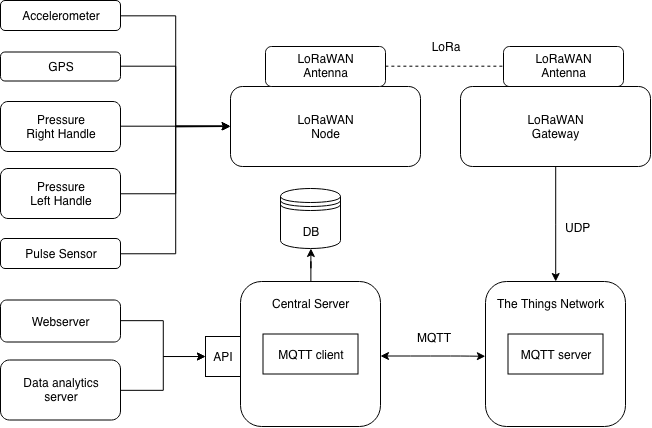
\includegraphics[width=1\linewidth]{gfx/architecture}
\caption{Proposed architecture}
\label{fig:image1}
\end{figure}

\section{Components and their interactions}


	\subsection{LoRaWAN node}
		Polls the sensors in predefined intervals and sends them through LoRaWAN every few minutes

	\subsection{LoRaWAN gateway}
		Receives LoRaWAN packets and relays them to "The Things Network" through the Semtech UDP protocol

	\subsection{The Things Network (TTN)}
		It is possible to have our gateway communicate directly with our server, but we decided to use TTN because it provides some very useful features out of the box, some of them being:

		\begin{itemize}
			\item Node authentication
			\item Packet deserialization
			\item Integration with MQTT, HTTP, Google Cloud, Amazon AWS and Azure
			\item Encryption
			\item Has thousands of registered gateways
		\end{itemize}

		TTN has become the standard in LoRaWAN applications, due to its unparalleled potencial for scalability, integration and security. In our case it deserializes the packets coming from the gateways and publishes them in an MQTT broker 

	\subsection{Server}
		The server will subscribe to the MQTT broker on TTN and store the information received from there, while also exposing an API that can be used, for example, to have other services process the data and display it to the interested parties

\section{Hardware Decisions}

	The proposed architecture can be realized in a number of ways, meaning we had to make the following choices:
	\begin{itemize}
		\item Use sensors with inbuilt LoRa functionality or use a single-board computer connected to sensors and LoRa transmitter?
		\item What hardware to use to interface with the sensors and act as the node?
		\item What hardware to use as LoRaWAN gateway?
	\end{itemize}


	\subsection{Single-board Computer vs Inbuilt LoRa Sensors:}

		We had the option of using a single-board computer (SBC) to interface with all of the sensors (Arduino or Rpi) or using sensors with inbuilt LoRaWAN capabilities.

		We summarized the haracteristics of sensors with inbuilt LoRaWAN as follows:
		\begin{itemize}
			\item They require little to no configuration and work out of the box. This means using them would grant us more time to we can focus on other parts of the project.
			\item Data can be sent at different rates for each sensor.
			\item They are much more expensive than standard sensors.
			\item They are bulkier than standard sensors, making them harder to fit into the walker.
			\item Their is low variety when it comes to such sensors in the market, limiting choice of vendor and sensors.
			\item Having several LoRaWAN transmitters instead of one would make the power consumption higher.
		\end{itemize}


		We summarized the following characteristics of SBCs:
		\begin{itemize}
			\item Fine grained control of the sensors
			\item We might want to do some preprocessing of the sensor data before sending it, which is possible with SBCs.
			\item Good amount of variety in the market allowing us a lot of choice.
		\end{itemize}

		We decided to go with an SBC because we value the flexibility provided by the vast array of sensors to choose from and the possibility to manually program them.



\subsection{Comparing Raspberry Pi and Arduino:}

	We then had the option of either using a Raspberry Pi or an Arduino. We summarized their characteristics as follows:

	Pi:
	\begin{itemize}
		\item Faster and more powerful processor
		\item Overhead of operating system, hdmi output, wifi/ethernet port, audio output, all of which take physical or disk space.
		\item More power consumption
	\end{itemize}

	Arduino:
	\begin{itemize}
		\item Easy to get up and running
		\item Easier to connect with analog sensors
		\item Lots of different models to choose from, meaning we can choose the one that best fits our goals
		\item Cheaper than the Raspberry Pi
		\item Smaller 
		\item No operating system, meaning we are closer to the hardware and have more control over the sensors
	\end{itemize}

	Due to the points mentioned above, especially due to its flexibility, and low power consumption, we decided to go with the arduino as the node.

	Due to its superior computational power, inbuilt networking capabilities, we decided to go with the Raspberry Pi as the gateway.

	Our reasoning is supported by the arguments put forward in \cite{postolache2011smart}.



\section{Experiments}
In order to test our hypothesis, we designed the following experiments:

	\subsection{Feasibility}
		In order to consider our hypothesis feasible we need to have some data being collected from sensors attached to a walker and sent through LoRaWAN to a remote server.

	\subsection{Normal Usage}
		In order to test the consistency and accuracy of our readings, the reliability of the whole system, its latency, and its energy consumption when in use, we have to use the walker and analyse what output we get. We will thus do two runs of 30 minutes, doing as much as possible to keep all the factors constant and save all the information we get. We can then use the sensor readings to find out our consistency and accuracy, the percentage of packets dropped for latency, the delay between them for latency and the energy used for energy consumption.

	\subsection{Idle Energy Consumption}
		We will leave the walker idle for around 12 hours while measuring its energy comsumption.
		We can then calculate how much energy the node consumes per hour both idle and in use (above experiment) and conclude how much it will last on common 9V batteries

	\subsection{Modularity}
		In order to test the modularity of the system, we will deliberately only integrate the GPS sensor in the testing phase of the project, this way we can measure how much time it takes and analyse the complications brought by doing so.

	\subsection{Scalability}
		Due to the fact that we only have one LoRaWAN hat for the Arduino, we are not able to have two setups running simultaneously, so we will re-register the arduino in "The Things Network" and re-upload the code to it, measuring how much time the process takes. We will do it once without practicing the process, and then one more time when we know exacly which steps to take.

	\subsection{Serviceability}
		We will get someone who is not a member of the team to disconnect random cables connecting the sensors to the node and we will then have another member get the system back up and running while measuring the time it takes.

	\subsection{Throughput}
		We will increase the ammount of bytes being sent by the node until 

	\subsection{Durability}
		Unfortunately, we don’t have enough time to test the durability of our system, so we’ll leave this as a possible improvement over our project



% \subsection{Consistency}
% To test consistency we will devise some usage scenarios and for each of them get 10 measurements. We will then compare the precision within and between scenarios by getting the variance.

% \subsection{Accuracy}
% In order to measure accuracy we need to find the difference between the measured value of each sensor and compare it to the true value. This means we need a test tailored to each sensor. For this, we will perform 10 measurements from each sensor and then find the standard deviation of the measured values from the true value.

% \subsection{Reliability}
% To measure reliability we will use the walker for 30 minutes and calculate the percentage of times the sensor data got stored in the server’s database

%%% Local Variables:
%%% mode: latex
%%% TeX-master: "../ClassicThesis"
%%% End:

%\chapter{Implementation}
\label{cha:implementation}

The final implementation of our system was follows:
\begin{figure}[h]
\centering
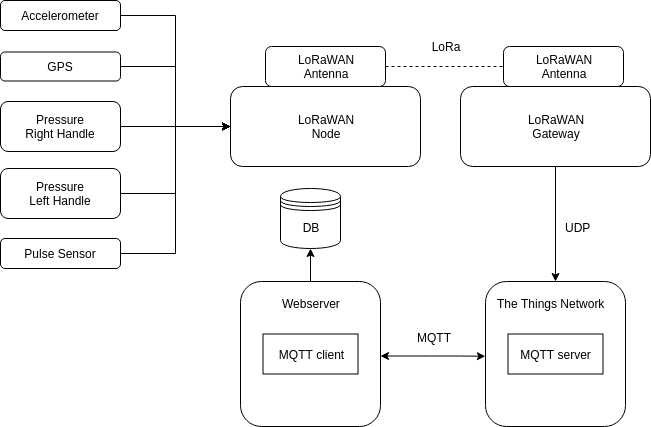
\includegraphics[width=0.7\linewidth]{gfx/implementation_arch}
\caption[]{Implemented Architecture}
\label{fig:implementation_arch}
\end{figure}

It differed from the overall design in the following ways:

We decided to use a webserver with an mqtt client and a database instead of a central server with API. We also decided to not implement the analytics server as part of the current project. We made these decisions prioritising the components that we needed to test our hypothesis. Since the presence or absence of a central server or analytics platform don't affect the parameters we need to test our hypothesis we decided to ignore them in the implementation part.

The implementation of each component of our system is described in details in the following subsections.



\subsection{Node:} 

\subsubsection{Hardware:}
The node consists of an Arduino Mega xxx with a Dragino LoRa hat xxx. The node is powered by a xxx battery pack. The node also consists of a breadboard, which contains two Analog to Digital converter and a gps sensor. The entire node setup is mounted on the front face of the lower left leg of the walker. The accelerometer is directly connected to the arduino and is mounted on the back face of the left leg of walker. Two pressure sensors are mounted on the handles of the walker and are connected to the A/D converters in the breadboard, which in turn are connected to the arduino. The pulse sensor is mounted on the left handle and is on top of a button and is directly connected to the arduino. The pulse sensor is only activated if the underlying button is pressed. 

The circuit diagram of the node is as follows:



\subsubsection{Software:}
The IDE used for writing and uploading the code was Visual Studio with Platform I/O extension. The Platform I/O simplified the process of uploading the code and monitoring the output of the arduino mega.

The libraries used were lmic, hal, SPI, SoftwareSerial, MPU9250 and HX711 along with the standard Arduino,stdlib and string library.

The code structure is as follows:
--Insert code tree here---

The main.cpp collects data in case of an event, converts the said data to bytes and sends it to a gateway using LoRaWAN. The main calls sensor specific functions to collect the data. 

Each LoRa packet contains the application id and key that is required by the things network.

\subsection{Pressure:}

\subsubsection{Hardware:}
For measuring pressure we used two HX711 sensors connected to the arduino via A/D converter module xxx. 

\subsubsection{Software:}
The sensor data was collected using HX711 library along with standard arduino library.

\subsection{Pulse:}


\subsection{Hardware:}
For pulse, we used the xxx sensor attached to a Lilypad button. The sensor was connected in a way that the pulse is read only when the button is pressed. This was done to prevent unnecessary read when the patient's finger is not on the sensor.


\subsubsection{Software:}
For reading the data from the sensor, simple analog read was used. This data is then processed to get average heart rate of the patient.



\subsection{Accelerometer:}

\subsection{Hardware:}
We used an MPU9250 accelerometer to measure whether the walker is moving or not.

\subsubsection{Software:}
The library used to read the accelerometer's output was sensor specific MPU9250 library. If the gyroscope reading from the accelerometer increased beyond a certain threshold, the walker was considered to be moving.


\subsection{GPS:}

\subsection{Hardware:}
For measuring GPS we used the xxx sensor.

\subsubsection{Software:}
The library used to read GPS data was SoftwareSerial. The read data was parsed to get the value of latitude and longitude, which were then converted to bytes.



\subsection{Gateway:}

\subsection{Hardware:}
We used raspberry pi 3+ along with dragino lora hat with gps model number 979854 for the gateway.
The gateway was made of a Raspberry Pi 3+ with a Dragino LoRa hat for Pi. The Pi was connected to a router which in turn was connected to the internet.


The circuit layout of the gateway is





\subsubsection{Software:}
the pi has a single chain packet forwarder code written in c, which forwards the packets it receives from the node to The Things Network's IP address. 


\subsection{The Things Network (TTN):}
The things network is an online website that we used to host our mqtt broker. We chose TTN because it's convinient, secure and very popular among the LoRaWAN community. We created an application in the TTN to act as our mqtt broker. We laso registered our gateway in TTN.

The application in TTN received packets from the gateway, converted them back from byte string to json and published them using the mqtt broker.


\subsection{Webserver:}
We created a webserver using the Django framework. It contained an mqtt client which subscribed to TTN. The mqtt borker was implemented using the paho mqtt library. The server then parsed the received data and stored them in a sqlite database. The database was then queried and the result was displayed on a webpage using django-tabular library.

We chose Django with sqlite for our server, because they allow quick prototyping and testing.

%%% Local Variables:
%%% mode: latex
%%% TeX-master: "../ClassicThesis"
%%% End:

%\chapter{Evaluation}
\label{cha:evaluation}

Having in mind our hypothesis: "Is it practical to monitor walkers and their users by sending data over LoRaWAN?"

The parameters of our system that have to be measured to test practicality were outlined in the introduction and the tests we intended to run were outlined in the "Design and Methodology" chapter.


\section{Normal Usage}

	\subsection{Pourpose}
	We are running this big experiment because measuring accuracy, consistency, reliability, latency and energy consumption, all have in common the fact that the best way to get data on these parameters is simply using the walker, so we devised this test, which has the goal of helping us simultaneously assess all the aforementioned quality parameters.

	\subsection{Expectations}
		\subsubsection{Consistency}
			We have different expectations, depending on the sensor:

			\begin{enumerate}
				\item Location: Our module's datasheet does not provide a precision threshold, so we don't know what to expect
				\item Heart Rate: The sensor we are using is very sensitive to noise and we have no way of keeping our heart rate constant when running the test, so we expect the readings to vary quite a lot.
				\item Movement: Since this is a boolean value, we expect it to be quite consistent, always reporting movement or no movement, given the same scenario.
				\item Pressure: We expect that if we manage to put constant force on the pressure sensors, they will give consistent readings
			\end{enumerate}

		\subsubsection{Accuracy}
			Again, each sensor can be said to be accurate if it meets conditions specific to it 

			\begin{enumerate}
				\item Location: According to the specification, the NEO 6M module should be accurate within 2 meters, so that is our expectation.
				\item Heart Rate: The sensor we are using is very sensitive to the pressure put on it and the thickness of the person's skin. We are also calculating the user's heart rate by processing the raw pulse data, so we don't expect much accuracy
				\item Movement: We are only using the accelerometer to measure if the walker is moving, so we expect an accuracy of 100\%, since we see no reason it would give an erroneous report
				\item Pressure: The pressure sensor we use does not provide an accuracy threshold, but from our preliminary usage it seems to be at least 95\% accurate
			\end{enumerate}

		\subsection{Reliability}
			The only failure we could see happening in this experiment would be LoRaWAN packets being sent from the node to the gateway being dropped, which doesn't seem to happen very often. We are thus expecting at least 90\% reliability

		\subsection{Latency}
			The air-time of LoRaWAN packets is dependent on the payload, the distance to the gateway, the spreading factor and much more, so it is hard for us to make an accurate prediction. We have nonetheless noticed, while building our system, that the time between packets is usually between 4 and 9 minutes, so we are expecting an average of around 6 minutes and a high standard deviation from the mean.
		\newline
		\newline
		\newline
		\subsection{Energy consumption}
			The power consumption of our components is as follows:

			\begin{table}[h]
				\begin{tabular}{@{}ll@{}}
					\toprule
					Sensor         & Max current draw (mA) \\ \midrule
					Pulse          & 4                     \\
					Pressure (x2)  & 3                     \\
					Accelerometer  & 0.5                   \\
					GPS            & 57                    \\
					LoRaWAN shield & 10                    \\
					Mega 2560      & 80                    \\
					Total          & 159                   \\ \bottomrule
				\end{tabular}
				\caption[Energy consumption Arduino]{Energy consumption Arduino}
				\label{tab:EnergyConsumption}
			\end{table}

			Based on this, we expect the current draw to be around 160mA

	\subsection{Parameters}
		We had on of our team's members use the walker normally for 30 minutes, while the information was coming in and stored in our server for analysis. There were only three details:

		\begin{itemize}
		  \item In order to test the accuracy of the heart rate, we had the team member testing the walker use an Iwatch for comparison, which is also not the most accurate of devices, but we don't have access to a better one
		  \item In order to test the consistency of the pressure sensor readings, we put an elastic band applying constant force on the right handle's sensor
		  \item In order to measure the current draw we used a USB Current Meter during the experiment
		\end{itemize}

	\subsection{Results}
		\subsection{Latency}

			Here are the times, in minutes and seconds, between packets:
			\begin{table}[h]
				\begin{tabular}{@{}lll@{}}
					Gap 	    &	First Run   & 	Second run 	 \\
					1st - 2nd 	&	7:35		& 	6:00     	 \\
					2nd - 3rd 	&	8:06    	& 	4:43         \\
					3rd - 4th 	&	6:47		& 	5:05         \\
					4th - 5th 	&	6:13    	& 	5:14         \\
					5th - 6th 	&	         	& 	4:24         \\
				\end{tabular}
				\caption[LoRaWAN latency]{LoRaWAN latency}
				\label{tab:Latency}
			\end{table}

			For the 1st run we got an average of 7:18

		\subsubsection{Heart Rate}
			First run:
			\begin{table}[h]
				\begin{tabular}{@{}ll@{}}
					Our Reading & IWatch Reading \\
					60          & 72             \\
					70          & 76             \\
					00          & 82             \\
					65          & 72             \\
					66          & 74            
				\end{tabular}
				\caption[Measuring heart rate first run]{Measuring heart rate first run}
				\label{tab:HeartRateFirst}
			\end{table}
			Second Run:
			\begin{table}[h]
				\begin{tabular}{@{}ll@{}}
					Our Reading & IWatch Reading \\
					72          & 64             \\
					00          & 64             \\
					62          & 72             \\
					65          & 70             \\
					61          & 65      		 \\      
					64          & 64
				\end{tabular}
				\caption[Measuring heart rate second run]{Measuring heart rate second run}
				\label{tab:HeartRateSecond}
			\end{table}

		\subsubsection{Pulse Sensor}

		\subsubsection{Energy consumption}
			The walker used 105 and 104 mAh during the first and second runs respectively. This means it was drawing a current of around 210mAh
	\subsection{Matching results and expectations}
		\subsubsection{Location}

		\subsubsection{Heart Rate}
			In both runs we got a reading of 0 in on of the measurements, so we will takes these as errors of the overall system and not take them into account in our statistical analysis.

			In the first run we got a mean average percentage error (MAPE) of 11.27, between this and the second run, we found an improvement that could be done to the algorithm, so we changed it for the second run, where we got a MAPE of 7.94. Given the constraints mentioned in our expectations, these results are better than we expected, perhaps because %34r come up with explanation

			We believe doing an analysis of the precision is not appropriate, since there was a gap of several minutes between measurements and the person was walking around, so there is no reason we should expect the heart rate to be constant.

		\subsubsection{Pressure}
			Regarding Accuracy, we had no way to get the real value of the pressure being applied on the handle while the walker is in use, so it doensn't seem like a relevant analysis to do. We have nonetheless previously tested the pressure sensors with a 1kg bag of rice, and both reported that exact value, so we can expect them to be similarly accurate while in use on the walker.

			We got a relative standard deviation of 8.27\% on the first run and 4.76\% on the second one, which is whithin our expectations. The deviations we see could be explained by the movement of the walker itself and/or changes in the position of the elastic band.

		\subsubsection{Movement}
			As expected, we got an accuracy of 100\% on the movement detection, and, since it is a boolean value, also a standard deviation of 0. Getting the movement status of the walker is a very simple measurement, so any result other than this would have been surprising.

		\subsubsection{Reliability}
			We 

		\subsubsection{Energy consumption}
			The walker consumed 30\% more than we expected, we think this could be because we are using two of the 5V pins, but it is most likely a factor we are not aware of and decided investigating it would be out of the scope our knowledge and most importantly this project.

\section{Idle Energy Consumption}

	\subsection{Pourpose}
		Most of the time, the walker will not be in use, so it is important to know how much energy it draws while idle
	\subsection{Expectations}

	\subsection{Parameters}
		We connected a USB Current Meter to the walker and left it idle for 5 minutes, while monitoring the current it was drawing
	\subsection{Results}
		The walker drew 0.2A throughout the 5 minutes, which
	\subsection{Matching results and expectations}

\section{Integrating the GPS sensor}
	\subsection{Pourpose}
	This experiment has the goal of figuring out how quickly a new sensor can be added to the walker. Our walker is a proof of concept for something bigger, so it is important to know how extensible it is.

	\subsection{Expectations}
	Having in consideration how much time it took us to mount, get readings, and send the current sensor's information, we expect to take around 1 or 2 days to integrate the GPS sensor into the system. 

	\subsection{Parameters}
	For this experiment, we had two of the team's members work exclusively on integrating the GPS sensor into the system. This consisted in mounting it on the walker, getting some readings, figuring out the best way to encode the data for sending over LoRaWAN, and then adapting the rest of the components to handle the latitude and longitude.

	\subsection{Results}
	Integrating GPS into the system ended up taking 2 whole days, not only was it hard to find a port layout which allowed all the sensors to work, but library support is also not very good, so after unsuccessfully trying to use external libraries, we ended up implementing it ourselves, which took some extra time.

	\subsection{Matching results and expectations}
	Integrating GPS into our system took as much time as we were roughly expecting, perhaps it is on the higher end of our expectation because of the usual delays that come with getting the right documentation for sensors and how they interplay with the other components. Two days doesn't seem like much having in consideration that repeating the process on new nodes would be much faster the following times.

	While performing this experiment, coincidentally, we noticed that when the GPS wasn't working and we wanted to use the walker for other tests, we had to remove it, so we could also say the system is modular in the sense that it is easy to remove sensors.

\section{Setting up the Arduino from scratch}

	\subsection{Pourpose}
		With this experiment we can get an idea of how scalable our system is, which is one of its most important features.
	\subsection{Expectations}
		We expect the first atempt to take around 4 minutes because we haven't registered a device in a while, but if the process is streamlined we expect it to take around 1:30 minutes, since it just requires navigating menues and slighly changing the node.
	\subsection{Parameters}
		We will, on the same computer, register a new device in The Things Network, change the node files to include its new authentication codes and upload them to the Arduino.
	\subsection{Results}
		The first atempt took 4:50 and the second one 01:02.
	\subsection{Matching results and expectations}
		The first atempt took a bit longer than expected, perhaps because we didn't remember very well how to navigate the menus and options on The Things Network. On the second run we were even faster than predicted, maybe because what takes the most time is simply navigating the menus, and after knowing exacly what do it is very fast. This experiment is not a complete demonstration of the scalability of our system, but it is the best we could come up with given the resources. It doesn't show how the system would handle several nodes in parallel but at least we know that the act of adding them would be quick.

\subsection{Disconnecting cables}

	\subsection{Pourpose}
		We wanted to have a test for accessing the serviceability of the walker, this will allow us to have an idea of how long the walker will take to be fixed when hardware problems arise.
	\subsection{Expectations}
		We expect the node to be fixed in around 2:30 minutes, which includes looking up the supposed layout and arranging the cables accordingly.
	\subsection{Parameters}
		One of the team members will disconnect 7 random cables from the node and another one will atempt to fix it.
	\subsection{Results}
		The node was back up and running in 1:22, having the first packet arriving on our server at 1:28.
	\subsection{Matching results and expectations}
		We overestimated the time it would take by a minute, we think this might be because the team member fixing the walker was the most familiar with the cabling and pin layout.

\section{Finding maximim throughput}

	\subsection{Pourpose}
		We dont intend to send much information, but it is nonetheless usefull knowing how much could theoretically be sent
	\subsection{Expectations}
		We have configured our system to be able to use a spreading factor between 7 and 12, which have a maximum payload of 222 and 51 bytes, respectively, so we are expecting any value in-between, but most likely one of these two, since they are the most commonly used.
	\subsection{Parameters}
		We will increase the payload by 
	\subsection{Results}
		We kept increasing, testing twice and decreasing the payload in the following fashion, until we found the maximum we could successfully send:

		\begin{table}[h]
			\begin{tabular}{@{}lllllllllll@{}}
				Payload (bytes) & 15  & 30  & 60 & 45  & 50  & 55 & 54 & 53 & 52 & 51  \\
				Success & yes & yes & no & yes & yes & no & no & no & no & yes
			\end{tabular}
		\end{table}

		For the payloads of 60, 55 and 54 bytes, the packets never arrived at ttn, for loads of 53 and 52 bytes, they arrived but the payload was not readable.

	\subsection{Matching results and expectations}
		The maximum payload we got was 51 bytes, which is one of the options we considered most likely. With this experiment we can be sure the system is using a spreading factor of 12, which provides a very long range, but a very small payload and thus small throughput.

%%% Local Variables:
%%% mode: latex
%%% TeX-master: "../ClassicThesis"
%%% ispell-dictionary: "british" ***
%%% mode:flyspell ***
%%% mode:auto-fill ***
%%% fill-column: 76 ***
%%% End:

%\chapter{Conclusion}
\label{cha:conclusion}

This work presents an analysis of the practicality of monitoring health parameters of walker users by sending data over LoRWAN. 

Our experiments indicate that if the node is optimized for its energy consumption, which we didn't have time to do, the LoRaWAN protocol, especially when integrated with a stack like \textit{The Things Network}, provides a very simple and streamlined way of connecting walkers that can send their information over very large distances, with high reliability and serviceability. 

We belive that with higher quality sensors, well integrated into the walker, the overall fidelity of the system would be very high, making it a viable way to monitor health parameters overtime, since latency is not an issue in that use case.

As for future work, having the arduino being capable of using LoRaWAN outside and switching to 



%%% Local Variables:
%%% mode: latex
%%% TeX-master: "../ClassicThesis"
%%% End:




%\part{Some Kind of Manual}
%\cleardoublepage%*******************************************************
% Publications
%*******************************************************
\pdfbookmark[1]{Publications}{publications}
\chapter*{Publications}\graffito{This is just an early --~and currently ugly~-- test!}
This might come in handy for PhD theses: some ideas and figures have appeared previously in the following publications:

%\noindent Put your publications from the thesis here. The packages \texttt{multibib} or \texttt{bibtopic} etc. can be used to handle multiple different bibliographies in your document.

\begin{refsection}[ownpubs]
    \small
    \nocite{*} % is local to to the enclosing refsection
    \printbibliography[heading=none]
\end{refsection}

\emph{Attention}: This requires a separate run of \texttt{bibtex} for your \texttt{refsection}, \eg, \texttt{ClassicThesis1-blx} for this file. You might also use \texttt{biber} as the backend for \texttt{biblatex}. See also \url{http://tex.stackexchange.com/questions/128196/problem-with-refsection}.
%\cleardoublepage%*******************************************************
% Acknowledgments
%*******************************************************
\pdfbookmark[1]{Acknowledgments}{acknowledgments}

\begin{flushright}{\slshape    
	It was the best of times, it was the worst of times,\\
	it was the age of wisdom, it was the age of foolishness,\\ 
	it was the epoch of belief, it was the epoch of incredulity,\\ 
	it was the season of Light, it was the season of Darkness,\\
	it was the spring of hope, it was the winter of despair\\ \medskip
    --- Charles Dickens - A Tale of Two Cities \cite{dickens}}
\end{flushright}



\bigskip

\begingroup
\let\clearpage\relax
\let\cleardoublepage\relax
\let\cleardoublepage\relax
\chapter*{Acknowledgments}

The above opening passage from 'A Tale of Two  Cities ' by Charles Dickens would describe excellently the highs and lows in this project. In the following we want to acknowledge people who mattered during this time.\\

First and for most, we would like to thank the Head of Health IT Lab at the Alexandra Institute Morten Kyng and our Professor Niels Olof Bouvin who is a member of the Participatory Information Technology department at the Aarhus University. Both gentlemen made this project in several ways possible. Without there constant support and able guidance, this project would not have been complete.\\

The door to Professor Olof's and Professor Doctor Morten Kyng's office was always open whenever we had troubles or a question about our research or writing. They consistently gave us different perspectives on each problem and helped in creating this final report which states the final results of our research.\\

We would also like to thank the experts that we have consulted along the way, namely Orbit Lab and ChomskyLab. 
Without their passionate participation and input regarding hardware, the project could not have been that successful.
\endgroup




%%************************************************
\chapter{Introduction}\label{ch:introduction}
%************************************************
This bundle for \LaTeX\ has two goals:
\begin{enumerate}
    \item Provide students with an easy-to-use template for their
    Master's
    or PhD thesis. (Though it might also be used by other types of
    authors
    for reports, books, etc.)
    \item Provide a classic, high-quality typographic style that is
    inspired by \citeauthor{bringhurst:2002}'s ``\emph{The Elements of
    Typographic Style}'' \citep{bringhurst:2002}.
\end{enumerate}
The bundle is configured to run with a \emph{full} 
MiK\TeX\ or \TeX Live\footnote{See the file \texttt{LISTOFFILES} for
needed packages. Furthermore, \texttt{classicthesis} 
works with most other distributions and, thus, with most systems 
\LaTeX\ is available for.} 
installation right away and, therefore, it uses only freely available 
fonts. (Minion fans can easily adjust the style to their needs.)

People interested only in the nice style and not the whole bundle can
now use the style stand-alone via the file \texttt{classicthesis.sty}.
This works now also with ``plain'' \LaTeX.

As of version 3.0, \texttt{classicthesis} can also be easily used with 
\mLyX\footnote{\url{http://www.lyx.org}} thanks to Nicholas Mariette 
and Ivo Pletikosić. The \mLyX\ version of this manual will contain
more information on the details.

This should enable anyone with a basic knowledge of \LaTeXe\ or \mLyX\ to
produce beautiful documents without too much effort. In the end, this
is my overall goal: more beautiful documents, especially theses, as I
am tired of seeing so many ugly ones.

The whole template and the used style is released under the
\acsfont{GNU} General Public License. 

If you like the style then I would appreciate a postcard:
\begin{center}
 André Miede \\
 Detmolder Straße 32 \\
 31737 Rinteln \\
 Germany
\end{center}
The postcards I received so far are available at:
\begin{center}
 \url{http://postcards.miede.de}
\end{center}
\marginpar{A well-balanced line width improves the legibility of
the text. That's what typography is all about, right?}
So far, many theses, some books, and several other publications have 
been typeset successfully with it. If you are interested in some
typographic details behind it, enjoy Robert Bringhurst's wonderful book.
% \citep{bringhurst:2002}.

\paragraph{Important Note:} Some things of this style might look
unusual at first glance, many people feel so in the beginning.
However, all things are intentionally designed to be as they are,
especially these:
\begin{itemize}
    \item No bold fonts are used. Italics or spaced small caps do the
    job quite well.
    \item The size of the text body is intentionally shaped like it
    is. It supports both legibility and allows a reasonable amount of
    information to be on a page. And, no: the lines are not too short.
    \item The tables intentionally do not use vertical or double
    rules. See the documentation for the \texttt{booktabs} package for
    a nice discussion of this topic.\footnote{To be found online at 
    \url{http://mirror.ctan.org/macros/latex/contrib/booktabs/}.}
    \item And last but not least, to provide the reader with a way
    easier access to page numbers in the table of contents, the page
    numbers are right behind the titles. Yes, they are \emph{not}
    neatly aligned at the right side and they are \emph{not} connected
    with dots that help the eye to bridge a distance that is not
    necessary. If you are still not convinced: is your reader
    interested in the page number or does she want to sum the numbers
    up?
\end{itemize}
Therefore, please do not break the beauty of the style by changing
these things unless you really know what you are doing! Please.

\paragraph{Yet Another Important Note:} Since \texttt{classicthesis}'
first release in 2006, many things have changed in the \LaTeX\ world. 
Trying to keep up-to-date, \texttt{classicthesis} grew and evolved 
into many directions, trying to stay (some kind of) stable and be 
compatible with its port to \mLyX. However, there are still many 
remains from older times in the code, many dirty workarounds here and 
there, and several other things I am absolutely not proud of (for 
example my unwise combination of \acsfont{KOMA} and 
\texttt{titlesec} etc.).
\graffito{An outlook into the future of \texttt{classicthesis}.}

Currently, I am looking into how to completely re-design and 
re-implement \texttt{classicthesis} making it easier to maintain and 
to use. As a general idea, \texttt{classicthesis.sty} should be 
developed and distributed separately from the template bundle itself. 
Excellent spin-offs such as \texttt{arsclassica} could also be 
integrated (with permission by their authors) as format configurations. 
Also, current trends of \texttt{microtype}, \texttt{fontspec}, etc. 
should be included as well. As I am not really into deep 
\LaTeX\ programming, 
I will reach out to the \LaTeX\ community for their expertise and help.


\section{Organization}
A very important factor for successful thesis writing is the
organization of the material. This template suggests a structure as
the following:
\begin{itemize}
    \marginpar{You can use these margins for summaries of the text
    body\dots}
    \item\texttt{Chapters/} is where all the ``real'' content goes in
    separate files such as \texttt{Chapter01.tex} etc.
 %  \item\texttt{Examples/} is where you store all listings and other
 %  examples you want to use for your text.
    \item\texttt{FrontBackMatter/} is where all the stuff goes that
    surrounds the ``real'' content, such as the acknowledgments,
    dedication, etc.
    \item\texttt{gfx/} is where you put all the graphics you use in
    the thesis. Maybe they should be organized into subfolders
    depending on the chapter they are used in, if you have a lot of
    graphics.
    \item\texttt{Bibliography.bib}: the Bib\TeX\ database to organize
    all the references you might want to cite.
    \item\texttt{classicthesis.sty}: the style definition to get this
    awesome look and feel. Does not only work with this thesis template
    but also on its own (see folder \texttt{Examples}). Bonus: works
    with both \LaTeX\ and \textsc{pdf}\LaTeX\dots and \mLyX.
    \item\texttt{ClassicThesis.tcp} a \TeX nicCenter project file.
    Great tool and it's free!
    \item\texttt{ClassicThesis.tex}: the main file of your thesis
    where all gets bundled together.
    \item\texttt{classicthesis-config.tex}: a central place to load all 
    nifty packages that are used. %In there, you can also activate 
    %backrefs in order to have information in the bibliography about 
    %where a source was cited in the text (\ie, the page number).
    
    \emph{Make your changes and adjustments here.} This means that you  
    specify here the options you want to load \texttt{classicthesis.sty} 
    with. You also adjust the title of your thesis, your name, and all 
    similar information here. Refer to \autoref{sec:custom} for more 
    information.
    
        This had to change as of version 3.0 in order to enable an easy 
        transition from the ``basic'' style to \mLyX.
    
\end{itemize}
In total, this should get you started in no time.


\clearpage
\section{Style Options}\label{sec:options}
There are a couple of options for \texttt{classicthesis.sty} that
allow for a bit of freedom concerning the layout:
\marginpar{\dots or your supervisor might use the margins for some
    comments of her own while reading.}
\begin{itemize}
    \item General:
        \begin{itemize}
            \item\texttt{drafting}: prints the date and time at the bottom of
    each page, so you always know which version you are dealing with.
    Might come in handy not to give your Prof. that old draft.
        \end{itemize}
    
    \item Parts and Chapters:
        \begin{itemize}
            \item\texttt{parts}: if you use Part divisions for your document,
    you should choose this option. (Cannot be used together with 
    \texttt{nochapters}.)
    
            \item\texttt{nochapters}: allows to use the look-and-feel with 
    classes that do not use chapters, \eg for articles. Automatically
    turns off a couple of other options: \texttt{eulerchapternumbers}, 
    \texttt{linedheaders}, \texttt{listsseparated}, and \texttt{parts}. 
    
        \item\texttt{linedheaders}: changes the look of the chapter
        headings a bit by adding a horizontal line above the chapter
        title. The chapter number will also be moved to the top of the
        page, above the chapter title.
    
        \end{itemize}

  \item Typography:
        \begin{itemize}
            \item\texttt{eulerchapternumbers}: use figures from Hermann Zapf's
            Euler math font for the chapter numbers. By default, old style
            figures from the Palatino font are used.
    
            \item\texttt{beramono}: loads Bera Mono as typewriter font. 
            (Default setting is using the standard CM typewriter font.)
            
            \item\texttt{eulermath}: loads the awesome Euler fonts for math. 
            Pala\-tino is used as default font.
    
            \item\texttt{pdfspacing}: makes use of pdftex' letter spacing
            capabilities via the \texttt{microtype} package.\footnote{Use 
            \texttt{microtype}'s \texttt{DVIoutput} option to generate
            DVI with pdftex.} This fixes some serious issues regarding 
            math formul\ae\ etc. (\eg ``\ss'') in headers. 
            
            \item\texttt{minionprospacing}: uses the internal \texttt{textssc}
            command of the \texttt{MinionPro} package for letter spacing. This 
            automatically enables the \texttt{minionpro} option, overriding
            \texttt{pdfspacing}.
    
        \end{itemize}  

    \item Table of Contents:
        \begin{itemize}
             \item\texttt{tocaligned}: aligns the whole table of contents on
            the left side. Some people like that, some don't.
            
            \item\texttt{dottedtoc}: sets pagenumbers flushed right in the 
            table of contents.

            \item\texttt{manychapters}: if you need more than nine chapters for 
        your document, you might not be happy with the spacing between the 
        chapter number and the chapter title in the Table of Contents. 
        This option allows for additional space in this context. 
        However, it does not look as ``perfect'' if you use
        \verb|\parts| for structuring your document.
            
        \end{itemize}
    
    \item Floats:
        \begin{itemize}
    \item\texttt{listings}: loads the \texttt{listings} package (if not 
    already done) and configures the List of Listings accordingly.
    
    \item\texttt{floatperchapter}: activates numbering per chapter for
    all floats such as figures, tables, and listings (if used). 
    
        \item\texttt{subfig}(\texttt{ure}): is passed to the \texttt{tocloft} 
        package to enable compatibility with the \texttt{subfig}(\texttt{ure}) 
        package. Use this option if you want use \texttt{classicthesis} with the
        \texttt{subfig} package.
        
%    \item\texttt{listsseparated}: will add extra space between table
%    and figure entries of different chapters in the list of tables or
%    figures, respectively. % Deprecated as of version 2.9.
        \end{itemize}    
 
%   \item\texttt{a5paper}: adjusts the page layout according to the
%    global \texttt{a5paper} option (\emph{experimental} feature).
%    \item\texttt{minionpro}: sets Robert Slimbach's Minion as the 
%    main font of the document. The textblock size is adjusted 
%    accordingly.    

   \end{itemize}
The best way to figure these options out is to try the different
possibilities and see what you and your supervisor like best.

In order to make things easier, \texttt{classicthesis-config.tex} 
contains some useful commands that might help you.


\section{Customization}\label{sec:custom}
%(As of v3.0, the Classic Thesis Style for \LaTeX{} and \mLyX{} share
%the same two \texttt{.sty} files.)
This section will show you some hints how to adapt 
\texttt{classicthesis} to your needs.

The file \texttt{classicthesis.sty}
contains the core functionality of the style and in most cases will
be left intact, whereas the file \texttt{classic\-thesis-config.tex}
is used for some common user customizations. 

The first customization you are about to make is to alter the document
title, author name, and other thesis details. In order to do this, replace
the data in the following lines of \texttt{classicthesis-config.tex:}%
\marginpar{Modifications in \texttt{classic\-thesis-config.tex}%
}

\begin{lstlisting}
    % **************************************************
    % 2. Personal data and user ad-hoc commands
    % **************************************************
    \newcommand{\myTitle}{A Classic Thesis Style\xspace} 
    \newcommand{\mySubtitle}{An Homage to...\xspace} 
\end{lstlisting}

Further customization can be made in \texttt{classicthesis-config.tex}
by choosing the options to \texttt{classicthesis.sty} 
(see~\autoref{sec:options}) in a line that looks like this:

\begin{lstlisting}
    \PassOptionsToPackage{eulerchapternumbers,drafting,listings,subfig,eulermath,parts}{classicthesis}
\end{lstlisting}

Many other customizations in \texttt{classicthesis-config.tex} are
possible, but you should be careful making changes there, since some
changes could cause errors.

Finally, changes can be made in the file \texttt{classicthesis.sty},%
\marginpar{Modifications in \texttt{classicthesis.sty}%
} although this is mostly not designed for user customization. The
main change that might be made here is the text-block size, for example,
to get longer lines of text.


\section{Issues}\label{sec:issues}
This section will list some information about problems using
\texttt{classic\-thesis} in general or using it with other packages.

Beta versions of \texttt{classicthesis} can be found at Bitbucket:
\begin{center}
    \url{https://bitbucket.org/amiede/classicthesis/}
\end{center}
There, you can also post serious bugs and problems you encounter.

\subsection*{Compatibility with the \texttt{glossaries} Package}
If you want to use the \texttt{glossaries} package, take care of loading it 
with the following options:
\begin{lstlisting}
    \usepackage[style=long,nolist]{glossaries}
\end{lstlisting}
Thanks to Sven Staehs for this information. 


\subsection*{Compatibility with the (Spanish) \texttt{babel} Package}
Spanish languages need an extra option in order to work with this template:
\begin{lstlisting}
    \usepackage[spanish,es-lcroman]{babel}
\end{lstlisting}
Thanks to an unknown person for this information (via the issue reporting). 


\paragraph{Further information for using \texttt{classicthesis} with Spanish (in addition to the above)}
In the file \texttt{ClassicThesis.tex} activate the language: 
\begin{lstlisting}
    \selectlanguage{spanish}
\end{lstlisting}
    
If there are issues changing \verb|\tablename|, \eg using this:
\begin{lstlisting}
    \renewcommand{\tablename}{Tabla}
\end{lstlisting}

This can be solved by passing \texttt{es-tabla} parameter to \texttt{babel}:
\begin{lstlisting}
    \PassOptionsToPackage{es-tabla,spanish,es-lcroman,english}{babel}
    \usepackage{babel}
\end{lstlisting}

But it is also necessary to set \texttt{spanish} in the \verb|\documentclass|.

Thanks to Alvaro Jaramillo Duque for this information. 


\subsection*{Compatibility with the \texttt{pdfsync} Package}
Using the \texttt{pdfsync} package leads to linebreaking problems with the \texttt{graffito} command. 
Thanks to Henrik Schumacher for this information. 



\section{Future Work}
So far, this is a quite stable version that served a couple of people
well during their thesis time. However, some things are still not as
they should be. Proper documentation in the standard format is still
missing. In the long run, the style should probably be published
separately, with the template bundle being only an application of the
style. Alas, there is no time for that at the moment\dots it could be
a nice task for a small group of \LaTeX nicians.

Please do not send me email with questions concerning \LaTeX\ or the
template, as I do not have time for an answer. But if you have
comments, suggestions, or improvements for the style or the template
in general, do not hesitate to write them on that postcard of yours.


\section{Beyond a Thesis}
The layout of \texttt{classicthesis.sty} can be easily used without the
framework of this template. A few examples where it was used to typeset 
an article, a book or a curriculum vitae can be found in the folder 
\texttt{Examples}. The examples have been tested with  
\texttt{latex} and \texttt{pdflatex} and are easy to compile. To 
encourage you even more, PDFs built from the sources can be found in the 
same folder. 
%(It might be necessary to adjust the path to 
%\texttt{classicthesis.sty} and \texttt{Bibliography.bib} within the 
%examples.)

%\lstinputlisting[caption=An Article]%
    %{Examples/classicthesis-article.tex}
    %
%\lstinputlisting[caption=A Book]%
    %{Examples/classicthesis-book.tex}
%
%\lstinputlisting[caption=A Curriculum Vit\ae]%
    %{Examples/classicthesis-cv.tex}


\section{License}
\paragraph{GNU General Public License:} This program is free software;
you can redistribute it and/or modify
 it under the terms of the \acsfont{GNU} General Public License as
 published by
 the Free Software Foundation; either version 2 of the License, or
 (at your option) any later version.

 This program is distributed in the hope that it will be useful,
 but \emph{without any warranty}; without even the implied warranty of
 \emph{merchant\-ability} or \emph{fitness for a particular purpose}.
 See the
 \acsfont{GNU} General Public License for more details.

 You should have received a copy of the \acsfont{GNU} General
 Public License
 along with this program; see the file \texttt{COPYING}.  If not,
 write to
 the Free Software Foundation, Inc., 59 Temple Place - Suite 330,
 Boston, MA 02111-1307, USA.

%*****************************************
%*****************************************
%*****************************************
%*****************************************
%*****************************************





%%% Local Variables:
%%% mode: latex
%%% TeX-master: "../ClassicThesis"
%%% End:

%\cleardoublepage

%\part{The Showcase}
%\section{Walker}

\subsection{GPS Module}
The GPS Module is used to analyse how sedentary the user is and what kinds of areas are most frequented by walker users and thus figure out what places might be worth investing in [\ref{fig:walkerpictures_gps}].
\begin{figure}[h!]
	\centering
	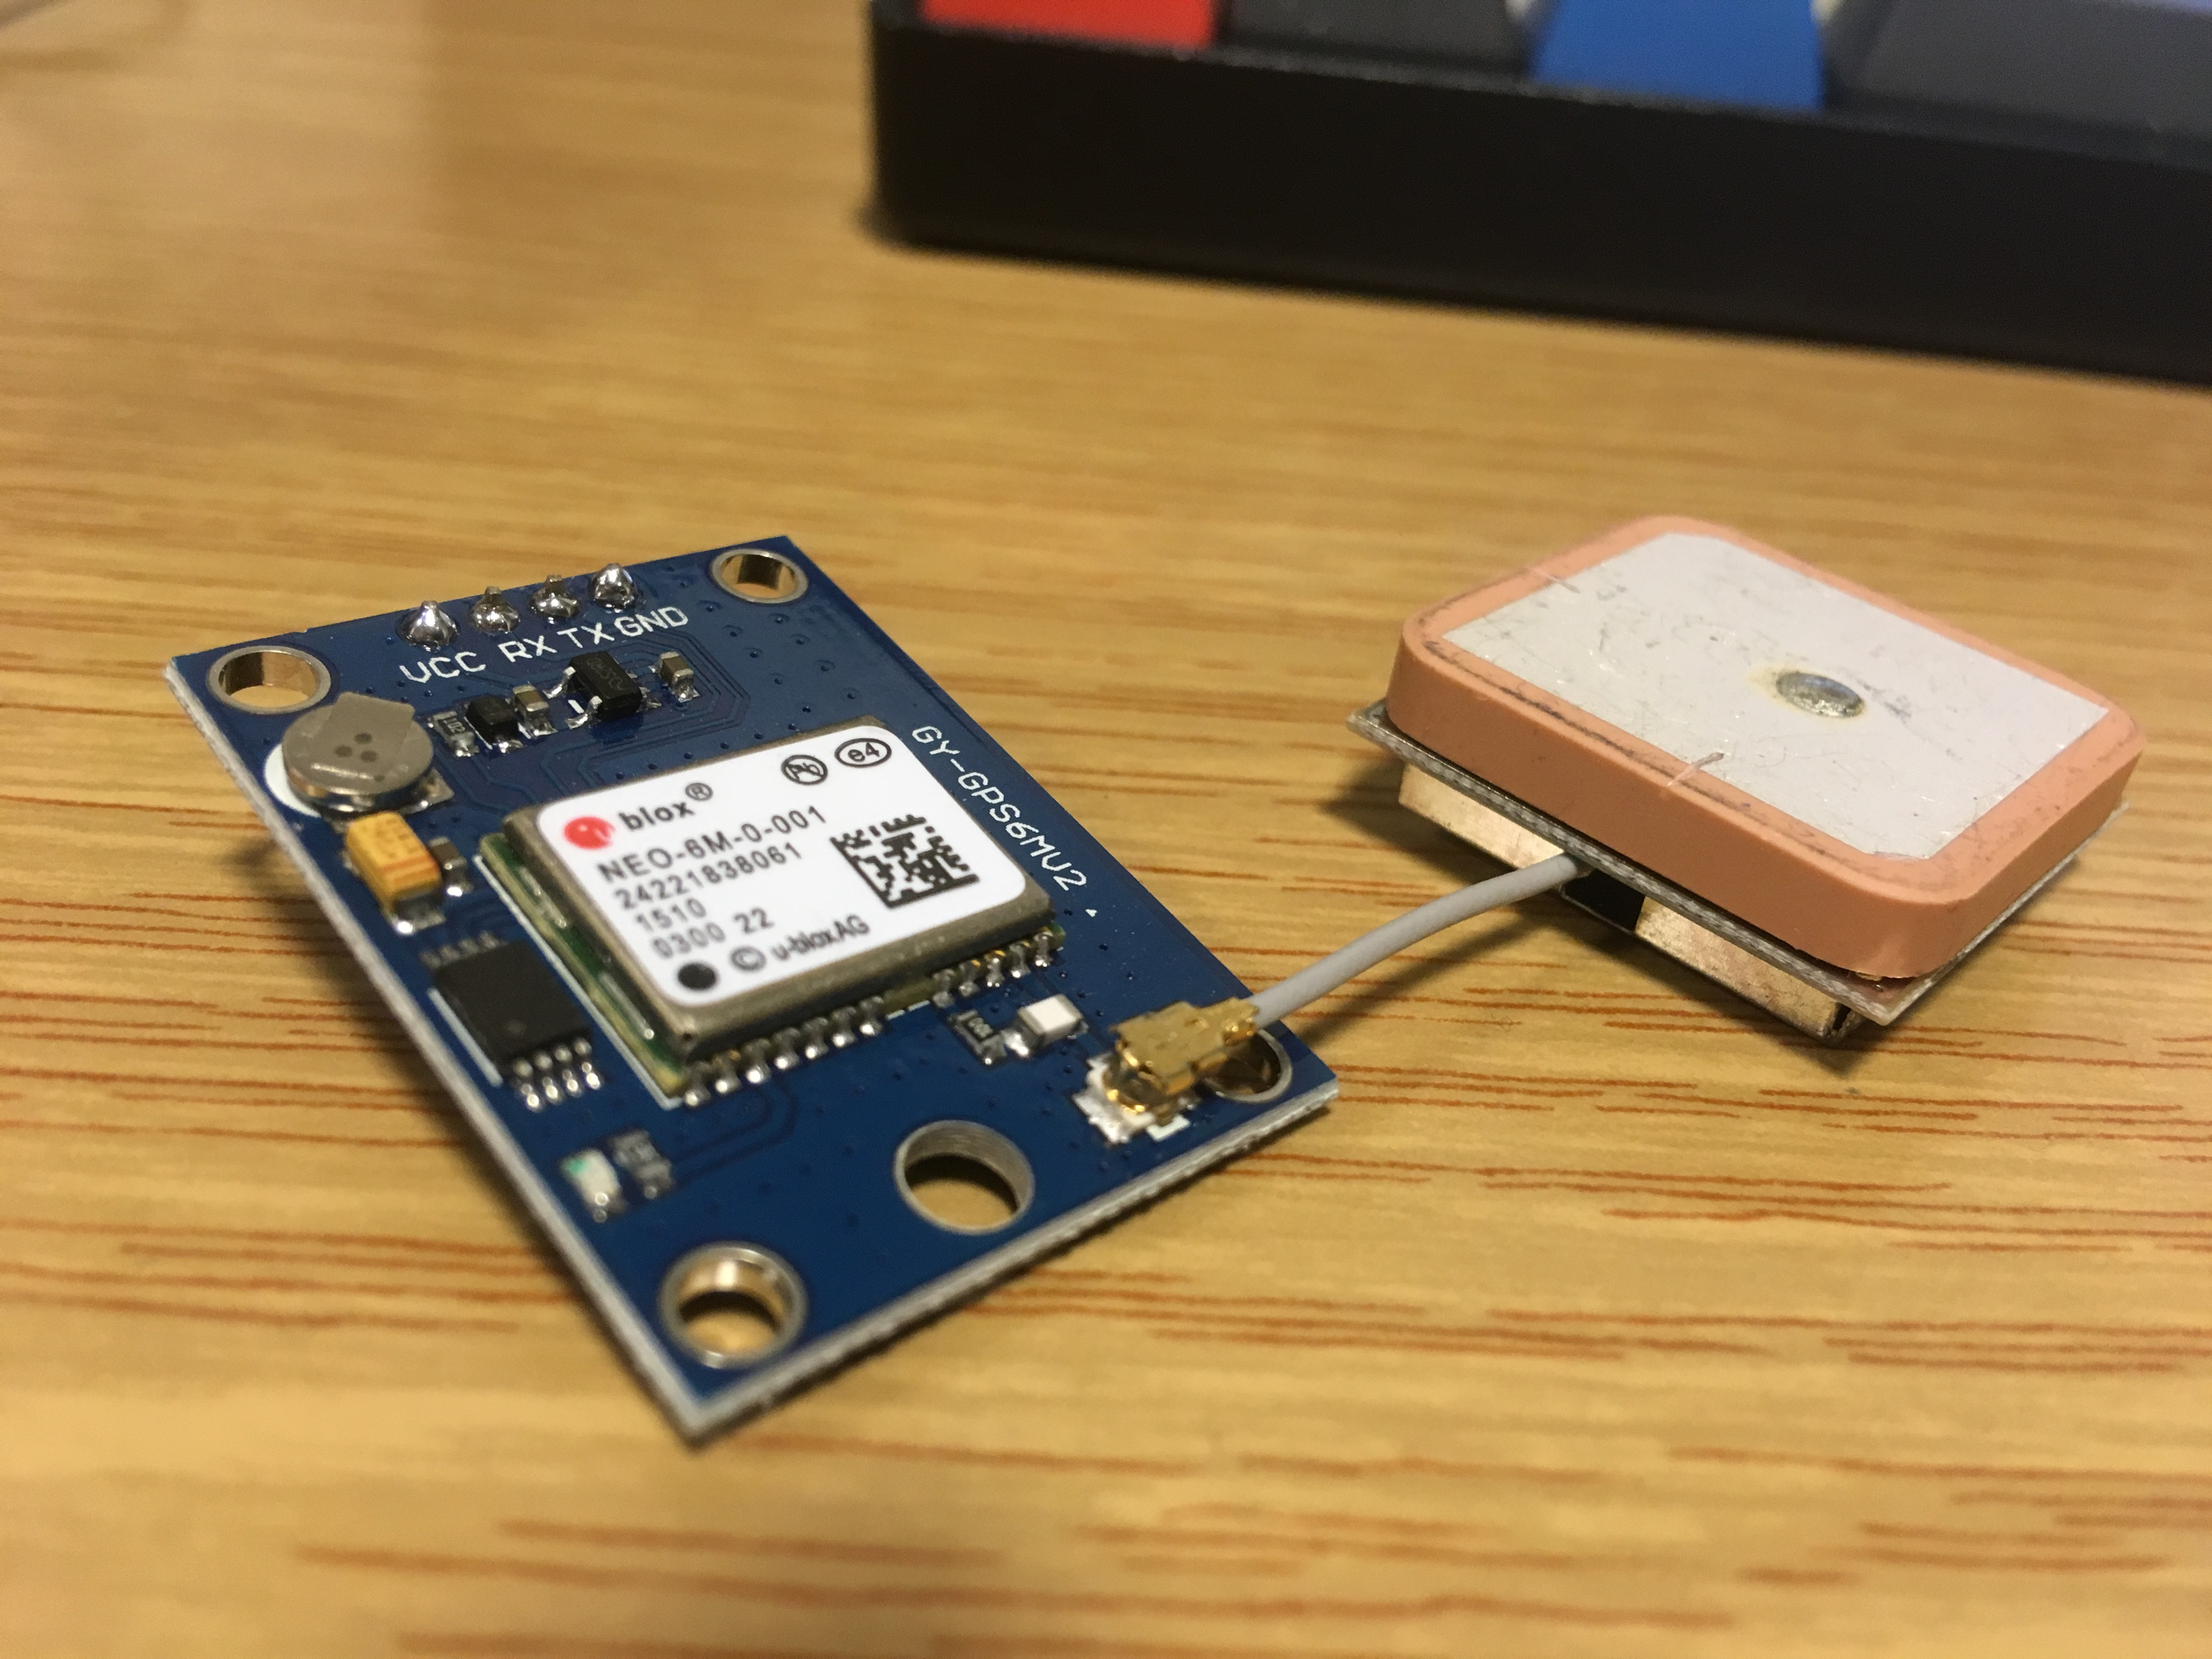
\includegraphics[width=0.7\linewidth]{gfx/walkerpictures/gps}
	\caption{Used GPS Module}
	\label{fig:walkerpictures_gps}
\end{figure}

\subsection{Heartrate Sensor}
This pulse sensor allows us to measure the user's heart rate [\ref{fig:walkerpictures_heartrate}].
\begin{figure}[h!]
	\centering
	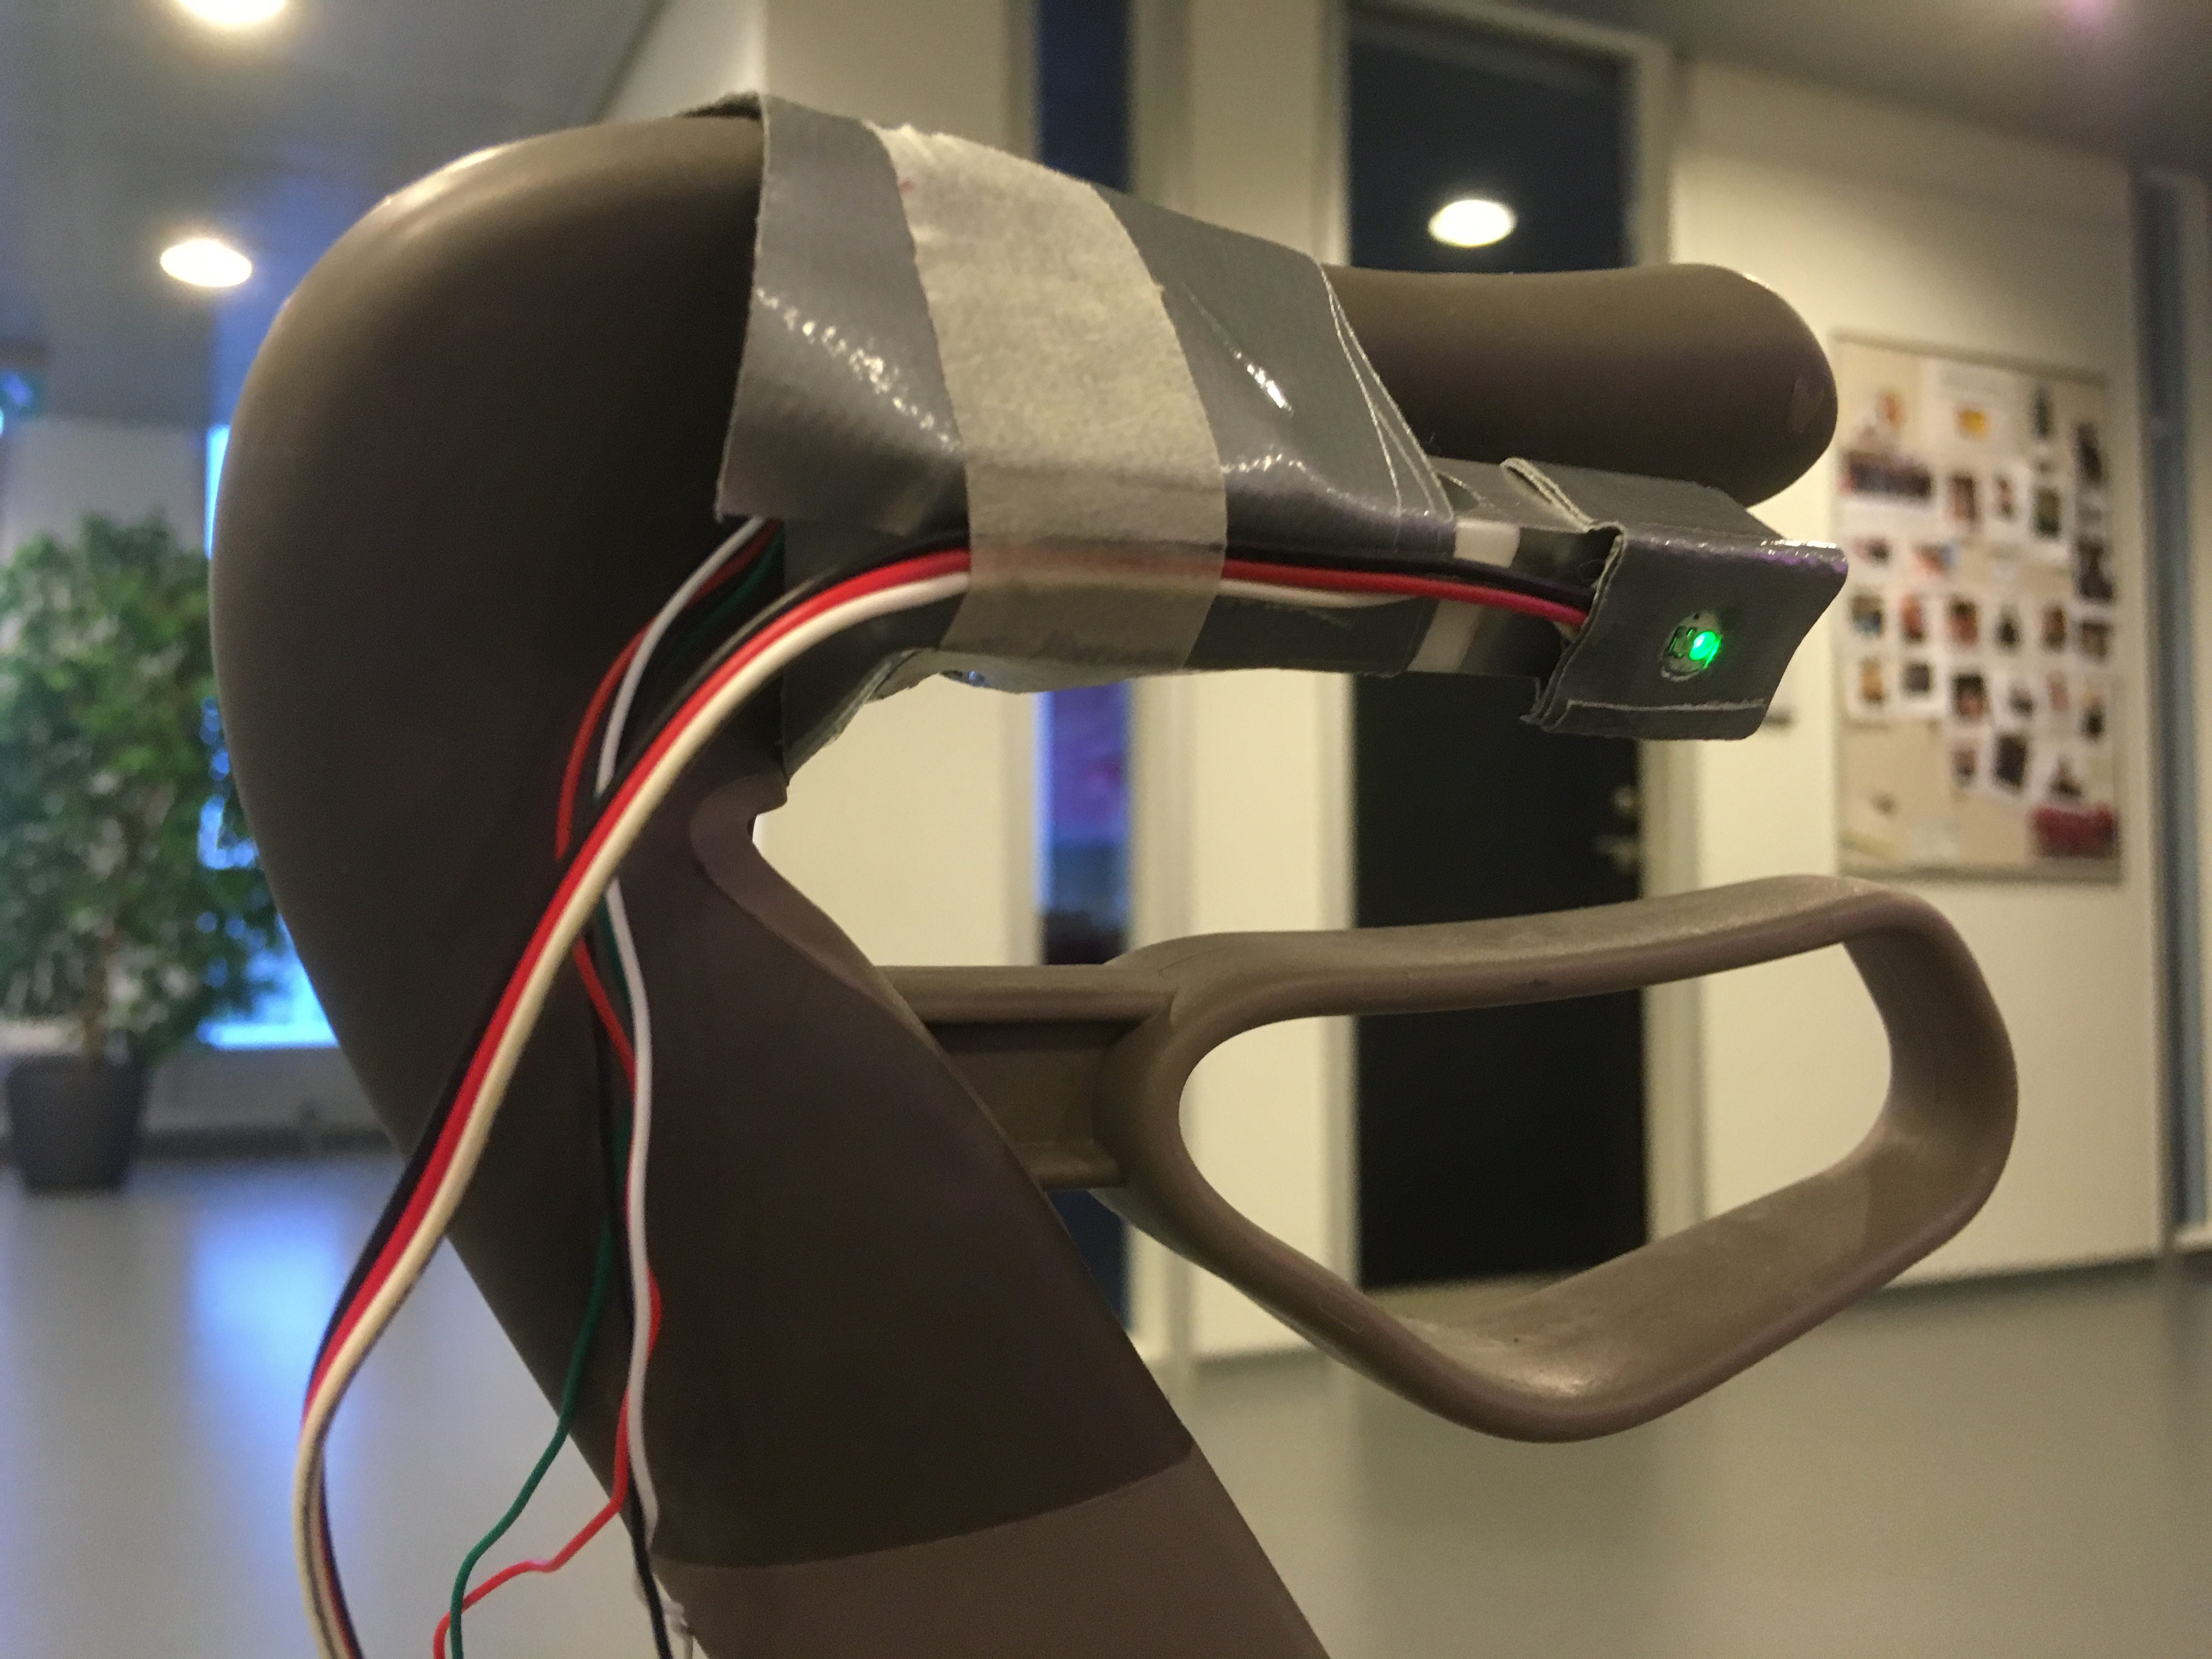
\includegraphics[width=0.7\linewidth]{gfx/walkerpictures/heartrate}
	\caption{Used Heartrate Sensor}
	\label{fig:walkerpictures_heartrate}
\end{figure}

\subsection{Movement Sensor}
The Movement Sensor allows us to measure the speed at which the user is walking. If we track both handles independently, together with the pressure measures, we can in a crude way analyse gait of the user [\ref{fig:walkerpictures_movement}].

\begin{figure}[h!]
	\centering
	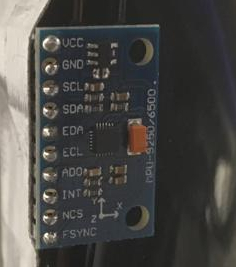
\includegraphics[width=0.7\linewidth]{gfx/walkerpictures/movement}
	\caption{Used Movement Sensor}
	\label{fig:walkerpictures_movement}
\end{figure}

\subsection{Pressure Sensors}
The Pressure Sensors allow us to track how much the user relies on the walker and how his/her grip strength changes over time [\ref{fig:walkerpictures_pressure}].

\begin{figure}[h!]
	\centering
	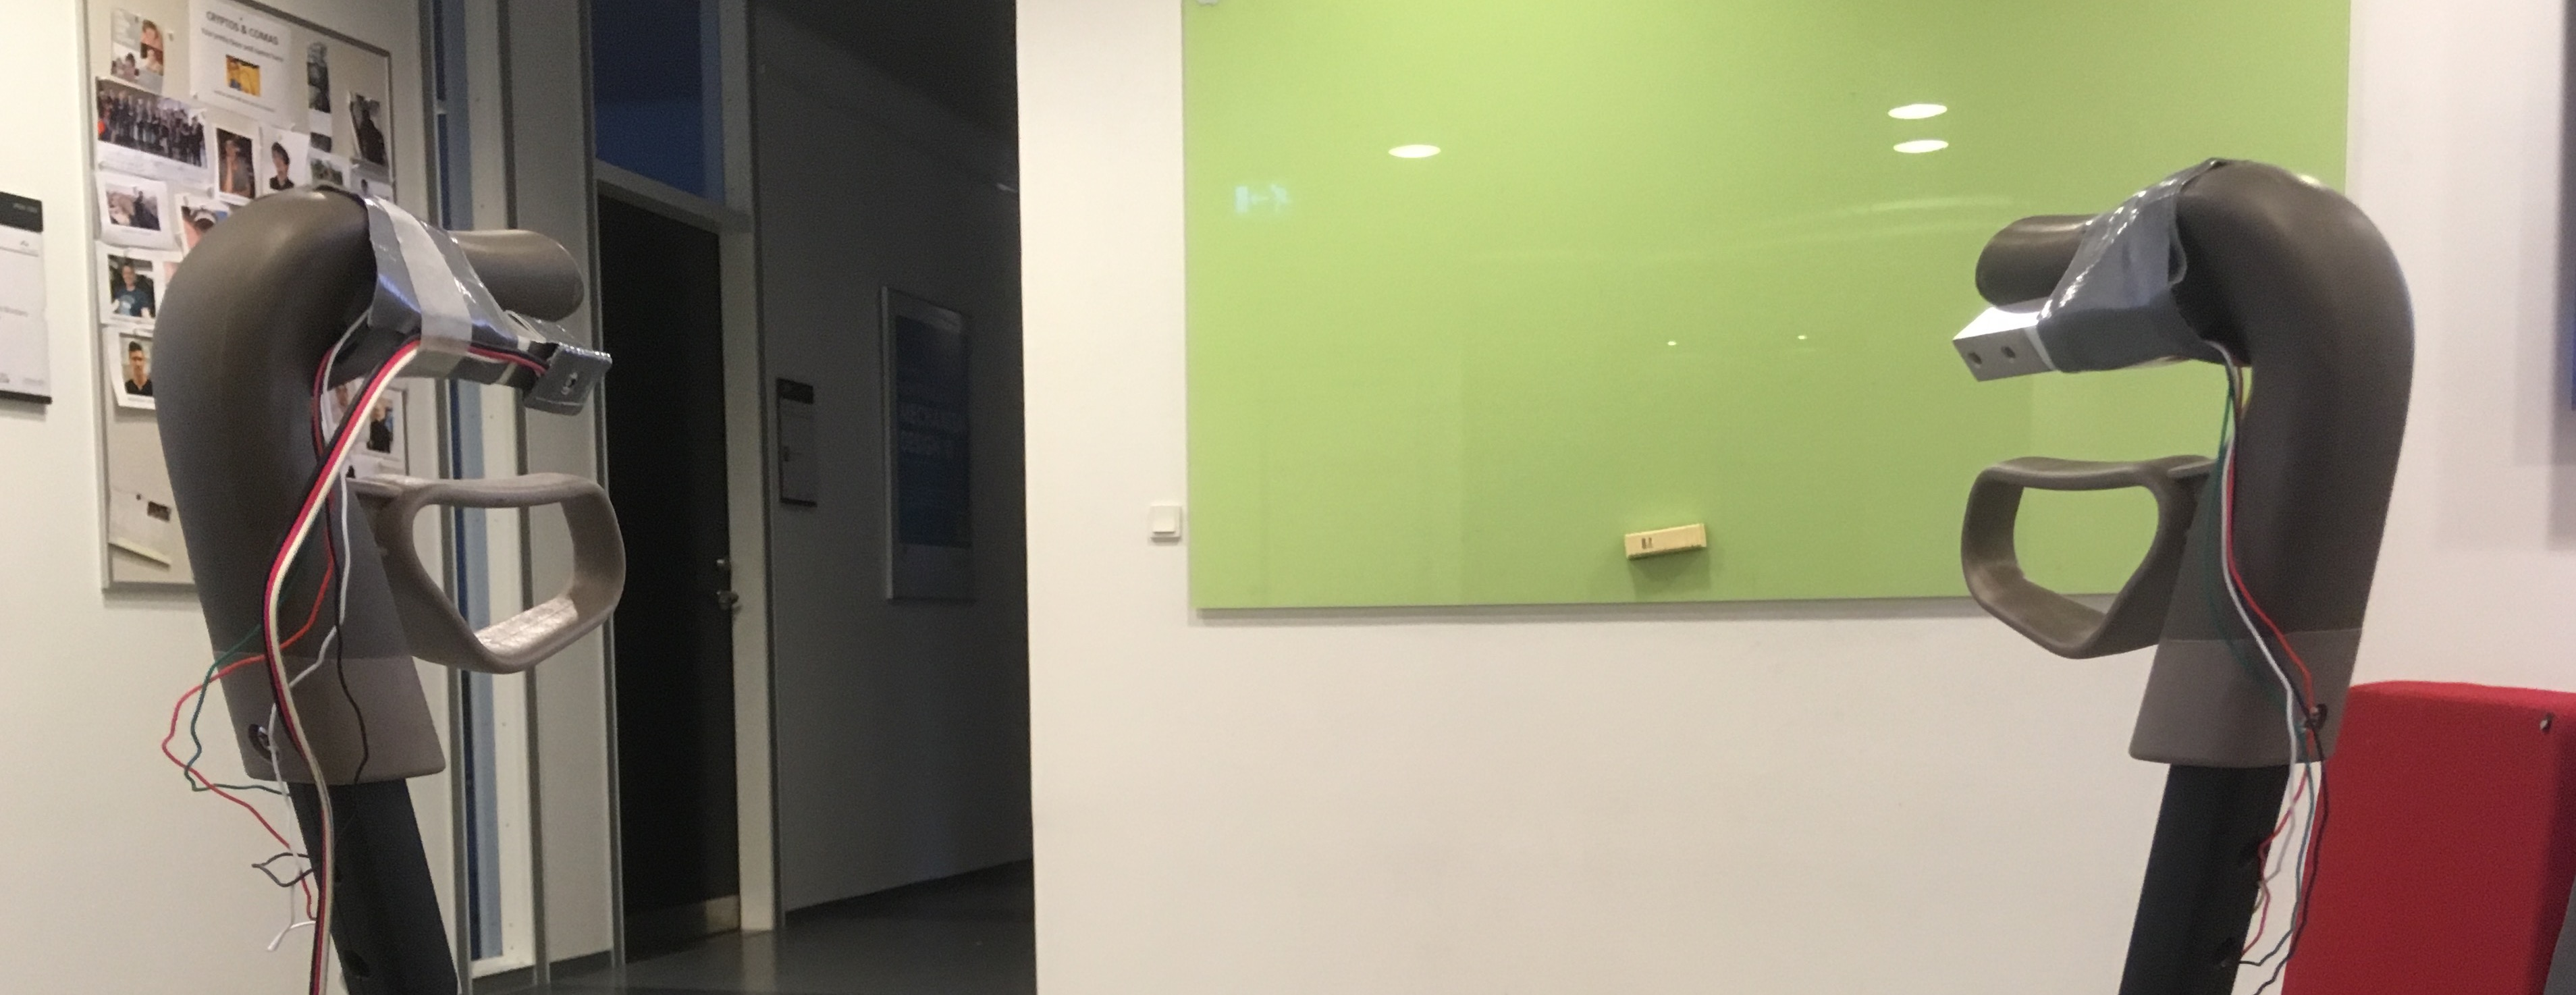
\includegraphics[width=0.7\linewidth]{gfx/walkerpictures/pressure}
	\caption{Used Pressure Sensors}
	\label{fig:walkerpictures_pressure}
\end{figure}


\subsection{LoRaWAN node}
A Arduino Mega with a LoRaWAN hat and connected to a battery, retrieving and sending sensor data [\ref{fig:walkerpictures_node}].
\begin{figure}[h!]
	\centering
	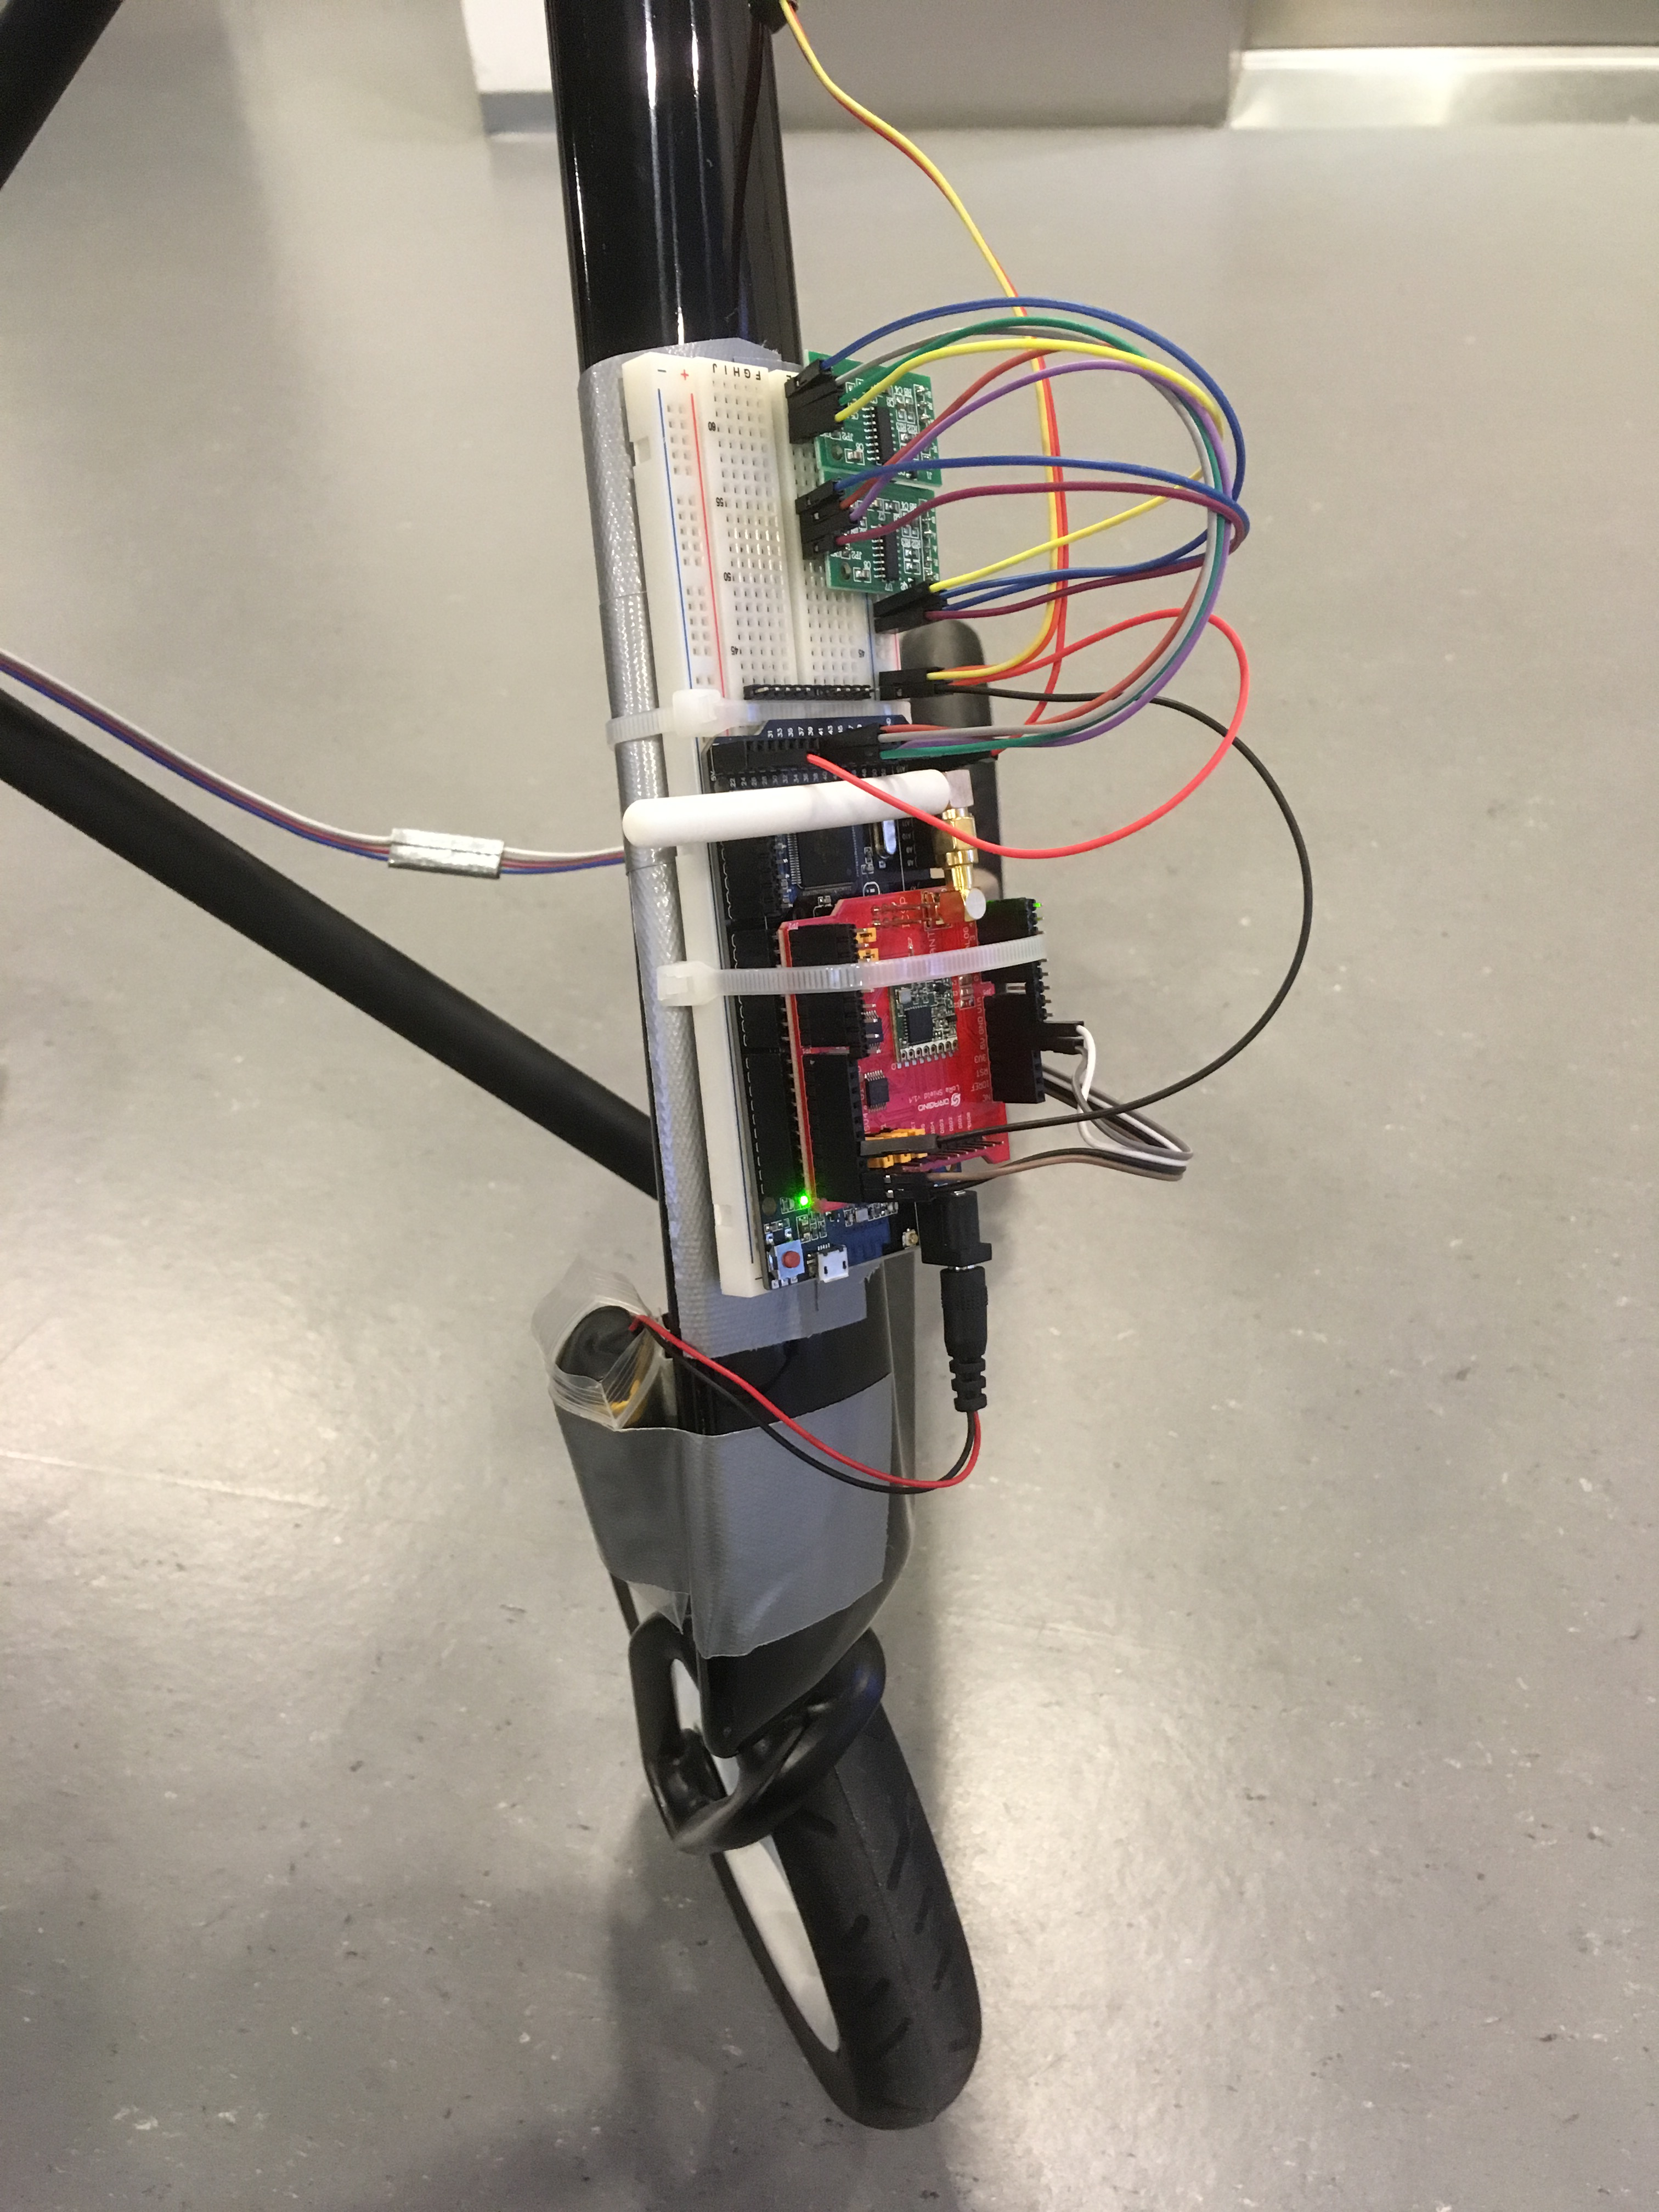
\includegraphics[width=0.7\linewidth]{gfx/walkerpictures/node}
	\caption{Used LoRaWAN node}
	\label{fig:walkerpictures_node}
\end{figure}
\newpage

\section{LoRaWAN gateway}
Raspberry Pi 3 with a LoRaWAN hat, forwarding LoRaWAN packets to The Things Network [\ref{fig:walkerpictures_gateway}].
\begin{figure}[h!]
	\centering
	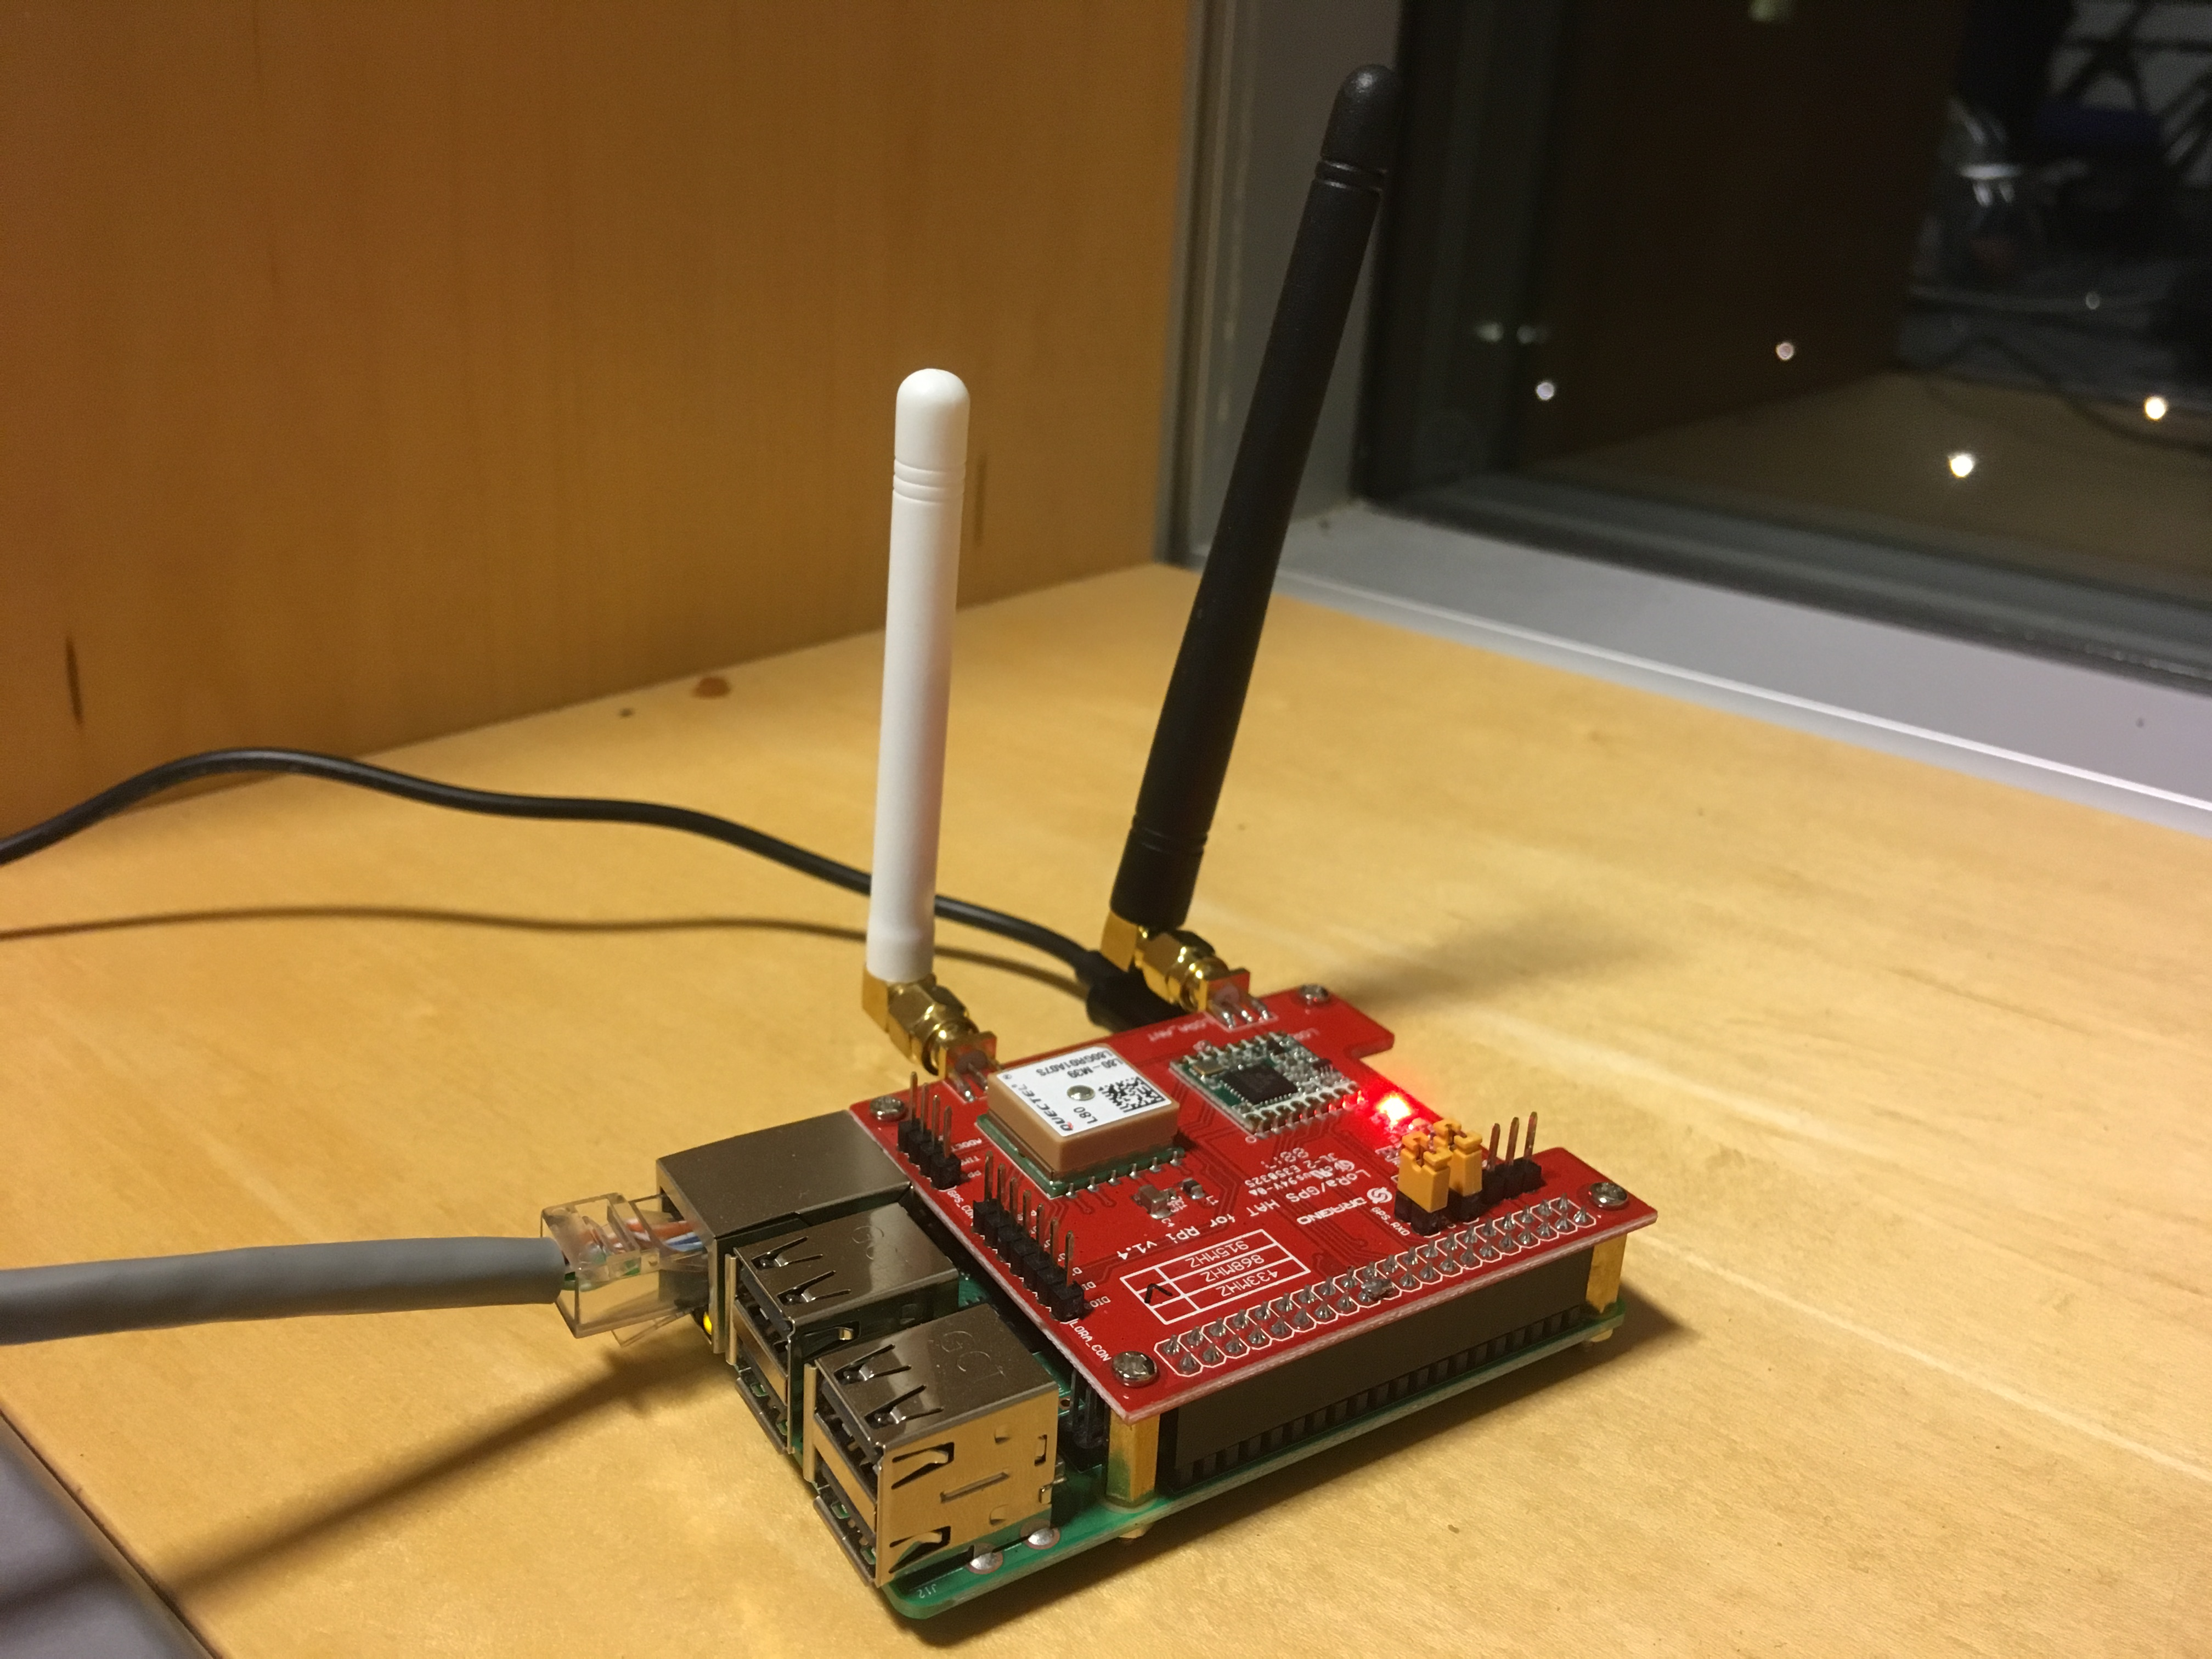
\includegraphics[width=0.7\linewidth]{gfx/walkerpictures/gateway}
	\caption{Used LoRaWAN gateway}
	\label{fig:walkerpictures_gateway}
\end{figure}

\section{Product Video}
In the following you can find a demonstration of the project:\\
https://vimeo.com/304645369


%\addtocontents{toc}{\protect\clearpage} % <--- just debug stuff, ignore
%%************************************************
\chapter{Math Test Chapter}\label{ch:mathtest} % $\mathbb{ZNR}$
%************************************************
Ei choro aeterno antiopam mea, labitur bonorum pri no. His no decore
nemore graecis. In eos meis nominavi, liber soluta vim cu. Sea commune
suavitate interpretaris eu, vix eu libris efficiantur.

\section{Some Formulas}
Due to the statistical nature of ionisation energy loss, large
fluctuations can occur in the amount of energy deposited by a particle
traversing an absorber element\footnote{Examples taken from Walter
Schmidt's great gallery: \\
\url{http://home.vrweb.de/~was/mathfonts.html}}.  Continuous processes
such as multiple
scattering and energy loss play a relevant role in the longitudinal
and lateral development of electromagnetic and hadronic
showers, and in the case of sampling calorimeters the
measured resolution can be significantly affected by such fluctuations
in their active layers.  The description of ionisation fluctuations is
characterised by the significance parameter $\kappa$, which is
proportional to the ratio of mean energy loss to the maximum allowed
energy transfer in a single collision with an atomic electron:
\graffito{You might get unexpected results using math in chapter or
section heads. Consider the \texttt{pdfspacing} option.}
\begin{equation}
\kappa =\frac{\xi}{E_{\textrm{max}}} %\mathbb{ZNR}
\end{equation}
$E_{\textrm{max}}$ is the maximum transferable energy in a single
collision with an atomic electron.
\[
E_{\textrm{max}} =\frac{2 m_{\textrm{e}} \beta^2\gamma^2 }{1 +
2\gamma m_{\textrm{e}}/m_{\textrm{x}} + \left ( m_{\textrm{e}}
/m_{\textrm{x}}\right)^2}\ ,
\]
where $\gamma = E/m_{\textrm{x}}$, $E$ is energy and
$m_{\textrm{x}}$ the mass of the incident particle,
$\beta^2 = 1 - 1/\gamma^2$ and $m_{\textrm{e}}$ is the electron mass.
$\xi$ comes from the Rutherford scattering cross section
and is defined as:
\begin{eqnarray*} \xi  = \frac{2\pi z^2 e^4 N_{\textrm{Av}} Z \rho
\delta x}{m_{\textrm{e}} \beta^2 c^2 A} =  153.4 \frac{z^2}{\beta^2}
\frac{Z}{A}
  \rho \delta x \quad\textrm{keV},
\end{eqnarray*}
where

\begin{tabular}{ll}
$z$          & charge of the incident particle \\
$N_{\textrm{Av}}$     & Avogadro's number \\
$Z$          & atomic number of the material \\
$A$          & atomic weight of the material \\
$\rho$       & density \\
$ \delta x$  & thickness of the material \\
\end{tabular}

$\kappa$ measures the contribution of the collisions with energy
transfer close to $E_{\textrm{max}}$.  For a given absorber, $\kappa$
tends
towards large values if $\delta x$ is large and/or if $\beta$ is
small.  Likewise, $\kappa$ tends towards zero if $\delta x $ is small
and/or if $\beta$ approaches $1$.

The value of $\kappa$ distinguishes two regimes which occur in the
description of ionisation fluctuations:

\begin{enumerate}
\item A large number of collisions involving the loss of all or most
  of the incident particle energy during the traversal of an absorber.

  As the total energy transfer is composed of a multitude of small
  energy losses, we can apply the central limit theorem and describe
  the fluctuations by a Gaussian distribution.  This case is
  applicable to non-relativistic particles and is described by the
  inequality $\kappa > 10 $ (\ie, when the mean energy loss in the
  absorber is greater than the maximum energy transfer in a single
  collision).

\item Particles traversing thin counters and incident electrons under
  any conditions.

  The relevant inequalities and distributions are $ 0.01 < \kappa < 10
  $,
  Vavilov distribution, and $\kappa < 0.01 $, Landau distribution.
\end{enumerate}


\section{Various Mathematical Examples}
If $n > 2$, the identity
\[
  t[u_1,\dots,u_n] = t\bigl[t[u_1,\dots,u_{n_1}], t[u_2,\dots,u_n]
  \bigr]
\]
defines $t[u_1,\dots,u_n]$ recursively, and it can be shown that the
alternative definition
\[
  t[u_1,\dots,u_n] = t\bigl[t[u_1,u_2],\dots,t[u_{n-1},u_n]\bigr]
\]
gives the same result.  

%*****************************************
%*****************************************
%*****************************************
%*****************************************
%*****************************************

%%% Local Variables:
%%% mode: latex
%%% TeX-master: "../ClassicThesis"
%%% End:




%\include{multiToC} % <--- just debug stuff, ignore for your documents
% ********************************************************************
% Backmatter
%*******************************************************
\appendix
%\renewcommand{\thechapter}{\alph{chapter}}
\cleardoublepage
%\part{Appendix}
%%********************************************************************
% Appendix
%*******************************************************
% If problems with the headers: get headings in appendix etc. right
%\markboth{\spacedlowsmallcaps{Appendix}}{\spacedlowsmallcaps{Appendix}}
\chapter{Appendix}


\section{Appendix Data}
In the following tables you can find all our test measurements:

\begin{table}[h!]
	\centering
	\begin{tabular}{@{}ll@{}}
		\toprule
		\textbf{Our Reading} & \textbf{IWatch Reading }\\ \midrule
		60          & 72             \\
		70          & 76             \\
		00          & 82             \\
		65          & 72             \\
		66          & 74             \\ \bottomrule
	\end{tabular}
	\caption[Measuring heart rate first run]{Measuring heart rate first run}
	\label{tab:HeartRateFirst}
\end{table}

\begin{table}[h!]
	\centering
	\begin{tabular}{@{}ll@{}}
		\toprule
		\textbf{Our Reading} & \textbf{IWatch Reading} \\ \midrule
		72          & 64             \\
		00          & 64             \\
		62          & 72             \\
		65          & 70             \\
		61          & 65      		 \\      
		64          & 64			 \\ \bottomrule
	\end{tabular}
	\caption[Measuring heart rate second run]{Measuring heart rate second run}
	\label{tab:HeartRateSecond}
\end{table}

\begin{table}[h!]
	\centering
	\begin{tabular}{@{}lllllll@{}}
		\toprule
		\textbf{Mesurements} & \textbf{1} & \textbf{2} & \textbf{3} & \textbf{4} & \textbf{5} & \textbf{6} \\ \midrule
		\textit{Run 1} & 0.45 & 0.39 & 0.45 & 0.38 & 0.40 &  \\
		\textit{Run 2} & 0.41 & 0.44 & 0.43 & 0.44 & 0.43 & 0.39 \\ \bottomrule
	\end{tabular}
	\caption[Measuring pressure first and second run]{Measuring pressure first and second run}
	\label{tab:PressureData}
\end{table}

\begin{table}[h!]
	\centering
	\begin{tabular}{@{}lllllllllll@{}}
		\toprule
		\textbf{Payload (bytes)} & 15  & 30  & 60 & 45  & 50  & 55 & 54 & 53 & 52 & 51  \\ \midrule
		\textbf{Success} & yes & yes & no & yes & yes & no & no & no & no & yes \\ \bottomrule
	\end{tabular}
	\caption[Payload testing LoraWAN]{Payload testing LoraWAN}
	\label{tab:LoraWanPayload}
\end{table}




%Ei solet nemore consectetuer nam. Ad eam porro impetus, te choro omnes
%evertitur mel. Molestie conclusionemque vel at, no qui omittam
%expetenda efficiendi. Eu quo nobis offendit, verterem scriptorem ne
%vix.


%%% Local Variables:
%%% mode: latex
%%% TeX-master: "../ClassicThesis"
%%% End:
%********************************************************************
% Other Stuff in the Back
%*******************************************************
%\cleardoublepage%********************************************************************
% Bibliography
%*******************************************************
% work-around to have small caps also here in the headline
\manualmark
\markboth{\spacedlowsmallcaps{\bibname}}{\spacedlowsmallcaps{\bibname}} % work-around to have small caps also
%\phantomsection 
\refstepcounter{dummy}
\addtocontents{toc}{\protect\vspace{\beforebibskip}} % to have the bib a bit from the rest in the toc
\addcontentsline{toc}{chapter}{\tocEntry{\bibname}}
\label{app:bibliography}
\printbibliography

%\cleardoublepage%*******************************************************
% Declaration
%*******************************************************
\refstepcounter{dummy}
\pdfbookmark[0]{Declaration}{declaration}
\chapter*{Declaration}
\thispagestyle{empty}
Put your declaration here.
\bigskip
 
\noindent\textit{\myLocation, \myTime}

\smallskip

\begin{flushright}
    \begin{tabular}{m{5cm}}
        \\ \hline
        \centering\myName \\
    \end{tabular}
\end{flushright}

%\cleardoublepage\pagestyle{empty}

\hfill

\vfill


\pdfbookmark[0]{Colophon}{colophon}
\section*{Colophon}
This document is a Project Report for the Building the Internet of Things with P2P and Cloud Computing subject by Niels Olof Bouvin from the University of Aarhus, Aarhus, in Denmark. 

\begin{table}[h]
	\begin{tabular}{ll}
		\textbf{} &  \\
		Title & \textbf{Remote Monitoring of Health Parameters Using smart walkers} \\
		&\\
		Version: & \noindent\finalVersionString\\
		&\\
		Date: & 07.12.2018 \\
		&\\
		Authors: & \myNameP, \myStudentIdP \\
		& \myNameH, \myStudentIdH \\
		& \myNameT, \myStudentIdT \\
		&\\
		University: & University of Aarhus \\
		& Åbogade 34\\
		& 8200 Aarhus\\
		& Faculty of Computer Science \\
		& Master of Science\\
		&\\
		First Supervisor: & Niels Olof Bouvin \\
		&\\
		Second Supervisor: & Michal Ratajský \\
		
	\end{tabular}\\
\end{table}
 
\bigskip

%Hermann Zapf's \emph{Palatino} and \emph{Euler} type faces (Type~1 PostScript fonts \emph{URW
%Palladio L} and \emph{FPL}) are used. The ``typewriter'' text is typeset in \emph{Bera Mono}, 
%originally developed by Bitstream, Inc. as ``Bitstream Vera''. (Type~1 PostScript fonts were made 
%available by Malte Rosenau and
%Ulrich Dirr.)

%\paragraph{note:} The custom size of the textblock was calculated
%using the directions given by Mr. Bringhurst (pages 26--29 and
%175/176). 10~pt Palatino needs  133.21~pt for the string
%``abcdefghijklmnopqrstuvwxyz''. This yields a good line length between
%24--26~pc (288--312~pt). Using a ``\emph{double square textblock}''
%with a 1:2 ratio this results in a textblock of 312:624~pt (which
%includes the headline in this design). A good alternative would be the
%``\emph{golden section textblock}'' with a ratio of 1:1.62, here
%312:505.44~pt. For comparison, \texttt{DIV9} of the \texttt{typearea}
%package results in a line length of 389~pt (32.4~pc), which is by far
%too long. However, this information will only be of interest for
%hardcore pseudo-typographers like me.%
%
%To make your own calculations, use the following commands and look up
%the corresponding lengths in the book:
%\begin{verbatim}
%    \settowidth{\abcd}{abcdefghijklmnopqrstuvwxyz}
%    \the\abcd\ % prints the value of the length
%\end{verbatim}
%Please see the file \texttt{classicthesis.sty} for some precalculated 
%values for Palatino and Minion.
%
%    \settowidth{\abcd}{abcdefghijklmnopqrstuvwxyz}
%    \the\abcd\ % prints the value of the length





% ********************************************************************
% Game Over: Restore, Restart, or Quit?
%*******************************************************
\end{document}
% ********************************************************************

%%% Local Variables:
%%% mode: latex
%%% TeX-master: t
%%% End:
